\documentclass[11pt,oneside]{article}

\usepackage[a4paper,margin=26mm,headheight=23pt]{geometry}
\usepackage[T1]{fontenc}
\usepackage[utf8]{inputenc}
\IfFileExists{libertinus.sty}{\usepackage{libertinus}}{\usepackage{lmodern}}
\usepackage{microtype}
\usepackage{amsmath,amssymb,amsthm,mathtools,mathrsfs}
\usepackage{bm}
\usepackage{booktabs,longtable,array,tabularx,multirow}
\usepackage{graphicx}
\usepackage{xcolor}
\usepackage{enumitem}
\usepackage{fancyhdr}
\usepackage{titlesec}
\usepackage{listings}
\usepackage{xurl}
\usepackage{tikz}
\usetikzlibrary{arrows.meta,positioning,calc,fit}
\usepackage[most]{tcolorbox}
\usepackage{hyperref}
\usepackage[nameinlink,noabbrev]{cleveref}

\definecolor{DeepBlue}{RGB}{30,58,95}
\definecolor{Teal}{RGB}{33,112,116}
\definecolor{Burgundy}{RGB}{125,49,62}
\definecolor{Gold}{RGB}{168,118,31}
\definecolor{LinkBlue}{RGB}{26,79,139}
\definecolor{SoftBlue}{RGB}{239,244,249}
\definecolor{SoftTeal}{RGB}{237,248,247}
\definecolor{SoftGold}{RGB}{252,248,235}
\definecolor{SoftRed}{RGB}{252,241,243}
\definecolor{RuleGray}{RGB}{193,201,209}
\definecolor{CodeGray}{RGB}{247,248,250}

\hypersetup{
  colorlinks=true,
  linkcolor=LinkBlue,
  citecolor=LinkBlue,
  urlcolor=LinkBlue,
  pdftitle={Dyadic Inverse Germs and Barnes--Rvachev Deconvolution},
  pdfauthor={Research synthesis based on Vladimir Reshetnikov's ProveIt corpus},
  pdfsubject={Fabius function, inverse Fabius function, Rvachev up-function, Appell and Barnes polynomials, Thue--Morse differences, q-Richardson recovery, reciprocal sinc poles, Lambert W},
  pdfkeywords={Fabius, Rvachev, Thue-Morse, Appell, Kabaya-Iri, Barnes Bernoulli, q-binomial, Richardson extrapolation, Lagrange inversion, Bell polynomial, Lambert W}
}

\pagestyle{fancy}
\fancyhf{}
\fancyhead[L]{\small\color{DeepBlue}Fabius--Rvachev inverse calculi}
\fancyhead[R]{\small\color{Teal}Frontier report}
\fancyfoot[C]{\small\thepage}
\renewcommand{\headrulewidth}{0.35pt}
\renewcommand{\headrule}{\hbox to\headwidth{\color{RuleGray}\leaders\hrule height \headrulewidth\hfill}}

\titleformat{\section}{\Large\bfseries\color{DeepBlue}}{\thesection}{0.7em}{}
\titleformat{\subsection}{\large\bfseries\color{DeepBlue}}{\thesubsection}{0.7em}{}
\titleformat{\subsubsection}{\normalsize\bfseries\color{DeepBlue}}{\thesubsubsection}{0.7em}{}
\setcounter{secnumdepth}{3}
\setcounter{tocdepth}{1}
\setlength{\emergencystretch}{3em}
\allowdisplaybreaks
\setlist[itemize]{leftmargin=2em,itemsep=0.25em,topsep=0.4em}
\setlist[enumerate]{leftmargin=2.4em,itemsep=0.25em,topsep=0.4em}

\newtheoremstyle{frontier}
  {0.7em}{0.7em}{\itshape}{}{\bfseries\color{DeepBlue}}{.}{0.55em}{}
\theoremstyle{frontier}
\newtheorem{theorem}{Theorem}[section]
\newtheorem{proposition}[theorem]{Proposition}
\newtheorem{lemma}[theorem]{Lemma}
\newtheorem{corollary}[theorem]{Corollary}
\newtheorem{conjecture}[theorem]{Conjecture}
\theoremstyle{definition}
\newtheorem{definition}[theorem]{Definition}
\newtheorem{algorithm}[theorem]{Algorithm}
\newtheorem{example}[theorem]{Example}
\theoremstyle{remark}
\newtheorem{remark}[theorem]{Remark}

\crefname{theorem}{theorem}{theorems}
\crefname{proposition}{proposition}{propositions}
\crefname{lemma}{lemma}{lemmas}
\crefname{corollary}{corollary}{corollaries}
\crefname{definition}{definition}{definitions}
\crefname{example}{example}{examples}
\crefname{algorithm}{algorithm}{algorithms}

\newtcolorbox{statusbox}[1][]{
  enhanced,breakable,colback=SoftBlue,colframe=DeepBlue,
  boxrule=0.65pt,arc=2pt,left=7pt,right=7pt,top=6pt,bottom=6pt,
  title={#1},fonttitle=\bfseries
}
\newtcolorbox{resultbox}[1][]{
  enhanced,breakable,colback=SoftTeal,colframe=Teal,
  boxrule=0.65pt,arc=2pt,left=7pt,right=7pt,top=6pt,bottom=6pt,
  title={#1},fonttitle=\bfseries
}
\newtcolorbox{cautionbox}[1][]{
  enhanced,breakable,colback=SoftGold,colframe=Gold,
  boxrule=0.65pt,arc=2pt,left=7pt,right=7pt,top=6pt,bottom=6pt,
  title={#1},fonttitle=\bfseries
}
\newtcolorbox{frontierbox}[1][]{
  enhanced,breakable,colback=SoftRed,colframe=Burgundy,
  boxrule=0.65pt,arc=2pt,left=7pt,right=7pt,top=6pt,bottom=6pt,
  title={#1},fonttitle=\bfseries
}

\lstdefinestyle{frontiercode}{
  basicstyle=\ttfamily\small,
  backgroundcolor=\color{CodeGray},
  frame=single,
  rulecolor=\color{RuleGray},
  columns=fullflexible,
  keepspaces=true,
  showstringspaces=false,
  breaklines=true,
  xleftmargin=0.7em,
  xrightmargin=0.7em,
  aboveskip=0.8em,
  belowskip=0.8em,
  keywordstyle=\color{DeepBlue}\bfseries,
  commentstyle=\color{Teal}
}

\newcommand{\R}{\mathbb R}
\newcommand{\C}{\mathbb C}
\newcommand{\Q}{\mathbb Q}
\newcommand{\Z}{\mathbb Z}
\newcommand{\N}{\mathbb N}
\newcommand{\e}{\mathrm e}
\newcommand{\ii}{\mathrm i}
\newcommand{\dd}{\,\mathrm d}
\newcommand{\GF}{\widetilde F}
\newcommand{\InvF}{G}
\newcommand{\Up}{\operatorname{up}}
\newcommand{\sinc}{\operatorname{sinc}}
\newcommand{\wt}{\operatorname{wt}_2}
\newcommand{\vtwo}{\nu_2}
\newcommand{\eps}{\varepsilon}
\newcommand{\ord}{\operatorname{ord}}
\newcommand{\supp}{\operatorname{supp}}
\newcommand{\coeff}[2]{[z^{#1}]\,#2}
\newcommand{\fall}[2]{#1^{\underline{#2}}}
\newcommand{\qpoch}[3]{(#1;#2)_{#3}}
\newcommand{\qbinom}[3]{\genfrac{[}{]}{0pt}{}{#1}{#2}_{#3}}
\newcommand{\Bell}{\mathcal B}
\newcommand{\BigO}{\mathcal O}
\newcommand{\littleo}{o}
\newcommand{\statusrepo}{\textsc{Repo}}
\newcommand{\statuslit}{\textsc{Prior}}
\newcommand{\statusnew}{\textsc{New}}

\begin{document}
\hypersetup{pageanchor=false}
\begin{titlepage}
\centering
\vspace*{1.25cm}
{\color{DeepBlue}\rule{\textwidth}{1.2pt}}\\[1.15cm]
{\Huge\bfseries Dyadic Inverse Germs and\\[0.25em]
Barnes--Rvachev Deconvolution\par}
\vspace{0.65cm}
{\Large New frontier results for the inverse Fabius function,\\
Kabaya--Iri polynomials, Thue--Morse differences, exact\\
$q$-Richardson recovery, reciprocal-sinc poles, and Lambert $W$\par}
\vspace{1.05cm}
{\color{Teal}\rule{0.82\textwidth}{0.75pt}}\\[0.95cm]
{\large A research synthesis based on the complete recursive LaTeX corpus in\\
\texttt{Analysis/FabiusFunction/docs} of Vladimir Reshetnikov's\\
\texttt{ProveIt} repository\par}
\vfill
\begin{minipage}{0.88\textwidth}
\small
\textbf{Research status.} The report distinguishes three levels of provenance.  Statements marked
\statusrepo\ are established in the audited repository; statements marked \statuslit\ are imported
from the external literature, notably the scaling-polynomial work of S.~L.~Lee; and statements
marked \statusnew\ are proved here and were not located explicitly in the 57-path repository
corpus by path, phrase, formula, and construction searches.  ``New'' is corpus-relative and is not
a claim of worldwide priority.  The external search found the Kabaya--Iri/Appell precursor, so the
novelty claims below are deliberately restricted to the dyadic inverse-germ, Barnes, Thue--Morse,
exact-recovery, logistic-duality, pole-asymptotic, and coefficient-threshold deductions.
\end{minipage}
\vfill
{\large 27 August 2026\par}
\vspace{0.8cm}
{\color{DeepBlue}\rule{\textwidth}{1.2pt}}
\end{titlepage}
\hypersetup{pageanchor=true}
\pagenumbering{roman}

\begin{abstract}
The Fabius--Rvachev system has two natural inverse problems.  The first is nonlinear: invert the
Fabius distribution function near a point.  The second is linear: invert averaging against the
Rvachev probability law on polynomials.  The repository develops the ingredients of both problems,
but not the common algebra that emerges when they are placed side by side.

For every interior dyadic point $x_0=a/2^N$, the Taylor series of $F$ terminates.  We show that the
Taylor germ of $G=F^{-1}$ at $F(x_0)$ is therefore the convergent algebraic inverse of a finite
rational polynomial.  The true inverse differs from this algebraic branch by a nonzero flat function.
At $x_0=1/4$ the algebraic shadow is a Catalan square-root branch, giving the exact all-order formula
\[
 G^{(m)}(5/72)=m!(-1)^{m-1}4^{m-1}C_{m-1}.
\]
This converts exact dyadic Fabius arithmetic into an explicit, Bell-polynomial and
Lagrange--B\"urmann calculus for the inverse.

For the linear problem, we begin from the known Kabaya--Iri scaling polynomials and recenter them
at the symmetric Rvachev law.  Their reciprocal moment generating function yields a centered Appell
sequence $A_n$.  We derive a Bernoulli-cumulant and Bell-polynomial calculus, and exhibit a new
dual random variable: an infinite dyadic sum of logistic variables whose characteristic function is
the reciprocal Rvachev moment generating function.  Consequently
$A_n(x)=\mathbb E(x+\ii Z)^n$, giving exact sign alternation of the Appell constants.

Finite dyadic convolution prefixes are identified exactly with normalized Barnes multiple Bernoulli
polynomials at the period vector $(1,1/2,\ldots,2^{1-N})$.  Applying the complete Thue--Morse
difference operator to these polynomials collapses them to one monomial, with a closed factor
$2^{-N(N-1)/2}\fall nN$.  Tail self-similarity then shows that every finite-prefix polynomial is an
\emph{exact} polynomial in $2^{-N}$ (or $4^{-N}$ after centering).  Gaussian $q$-binomial Lagrange
weights therefore recover the infinite Kabaya--Iri polynomial exactly after finitely many prefix
levels; this is Richardson extrapolation without a remainder.

Finally, the reciprocal moment generating function is meromorphic with poles at $2\pi\ii n$ of
order $\vtwo(n)+1$.  We transfer the full $2$-adic zero divisor of the infinite sinc product into
large-degree asymptotics of the Appell constants.  The first three pole shells give an explicit
three-term expansion with a polynomial correction from the double pole at $4\pi\ii$.  Stirling
inversion then produces a second, coefficient-theoretic role for the Lambert $W$ function: the first
index at which the Appell constants exceed a prescribed size is
$\log X/(2W(\log X/(2\pi e)))+O(1)$.
\end{abstract}

\begingroup
\footnotesize
\setlength{\parskip}{0pt}
\tableofcontents
\endgroup
\clearpage
\pagenumbering{arabic}

\section{Scope, corpus audit, and result boundary}
\label{sec:scope}

\subsection{What was audited}

The target tree is not a single manuscript.  It contains a primary exposition, a mathematical
glossary, a Lean walkthrough, a consolidated frontier volume, an active Thue--Morse formula atlas,
twelve Fourier-decay dossiers, seven source-paper transcriptions, and thirty-two frozen historical
sources.  The recursive ledger contains 57 distinct \texttt{.tex} paths: 25 living paths and 32 archive
paths.  The complete path list is reproduced in \cref{app:inventory}.

The overlap audit used four complementary tests.
\begin{enumerate}
\item Current successors were read at source level, including the main Fabius--Rvachev exposition,
      the frontier volume, the formula atlas, the inverse supplement, the $q$-special-function
      exposition, the Fourier-decay synthesis, and the latest interpolation/extrapolation reports.
\item Frozen versions were treated as prior art, not discarded as obsolete.  Revision chains and
      archive provenance maps were used to identify claims unique to earlier drafts.
\item Exact phrase and formula searches were run for Appell, Sheffer, umbral, Barnes--Bernoulli,
      multiple Bernoulli, mean-value inversion, polynomial deconvolution, and the new pole and
      inverse-germ formulas.
\item A targeted literature search was made after the repository audit.  It found Lee's 2009
      construction of the Kabaya--Iri biorthogonal Appell polynomials for the up-function.  The
      report therefore imports that construction rather than relabeling it as new.
\end{enumerate}

\begin{statusbox}[Nonduplication boundary]
The repository already contains extensive work on exact dyadic Fabius values, the global signed
extension, terminating Taylor series, the totalized inverse, inverse endpoint asymptotics, Gaussian
$q$-binomial interpolation, Thue--Morse Prouhet cancellation, finite splines, sharp convolution
errors, Bernoulli cumulants, Bell-polynomial saddle expansions, logarithmic sinc-product
Richardson extrapolation, phase-locked Lambert nodes, Fourier zero divisors, arithmetic rays, and a
higher-rank Pascal--Rvachev hierarchy.  None of those results is reproved as a purported novelty.
The new contribution is the set of compositions among them listed in \cref{tab:result-map}.
\end{statusbox}

\subsection{Result map}

\begin{table}[htbp]
\centering
\small
\begin{tabularx}{\textwidth}{@{}p{0.25\textwidth}X p{0.12\textwidth}@{}}
\toprule
Object & Principal statement & Status \\
\midrule
Dyadic inverse germ
& The Taylor series of $G$ at $F(a/2^N)$ is the algebraic inverse of a finite rational polynomial;
  the discrepancy from $G$ is nonzero and flat. & \statusnew \\
Catalan point
& $G^{(m)}(5/72)=m!(-1)^{m-1}4^{m-1}C_{m-1}$. & \statusnew \\
Kabaya--Iri sequence
& $e^{xt}/L(t)=\sum P_n(x)t^n/n!$ and biorthogonality to derivatives of the up/Fabius density. & \statuslit \\
Centered Appell sequence
& $A_n(x)=2^nP_n((x+1)/2)$, with Bernoulli cumulants and Bell constants. & derived \\
Logistic dual
& $1/M(t)$ is the characteristic function of a dyadic logistic series, so
  $A_n(x)=\mathbb E(x+\ii Z)^n$. & \statusnew \\
Dyadic Barnes prefix
& Finite-prefix polynomials are normalized Barnes multiple Bernoulli polynomials at a geometric period vector. & \statusnew \\
Thue--Morse operator
& A complete binary signed difference of a finite-prefix Appell polynomial collapses exactly to a monomial. & \statusnew \\
Exact $q$-Richardson recovery
& The limiting Appell polynomial is recovered exactly from finitely many convolution-prefix levels by Gaussian $q$-binomial weights. & \statusnew \\
Reciprocal-sinc poles
& Pole order $\vtwo(n)+1$ becomes a degree-$\vtwo(n)$ polynomial correction in the large-degree Appell constants. & \statusnew \\
Lambert threshold
& The first coefficient above size $X$ has index $\log X/(2W(\log X/(2\pi e)))+O(1)$. & \statusnew \\
\bottomrule
\end{tabularx}
\caption{The result boundary used throughout the report.}
\label{tab:result-map}
\end{table}

\subsection{Why the two inverse problems belong together}

Let $\mu$ be the probability law of the Fabius random variable $X$, and let $\nu$ be the centered
Rvachev law of $Y=2X-1$.  There are two different inverses:
\begin{align*}
\text{nonlinear inverse:}\qquad &F(x)=y \longmapsto x=G(y),\\
\text{linear polynomial inverse:}\qquad
 &(\mathcal T_\nu p)(x):=\int p(x+y)\,\nu(\dd y)
 \longmapsto \mathcal T_\nu^{-1}x^n=A_n(x).
\end{align*}
The first is governed by compositional inversion and therefore by Lagrange--B\"urmann and partial
Bell polynomials.  The second is governed by reciprocal exponential generating functions and
therefore by Appell, Barnes, Bernoulli, and complete Bell polynomials.  Dyadic self-similarity makes
both inverse calculi finite at special scales: the nonlinear Taylor jet terminates at a dyadic point,
and the finite convolution prefix is a finite Barnes product.

\begin{center}
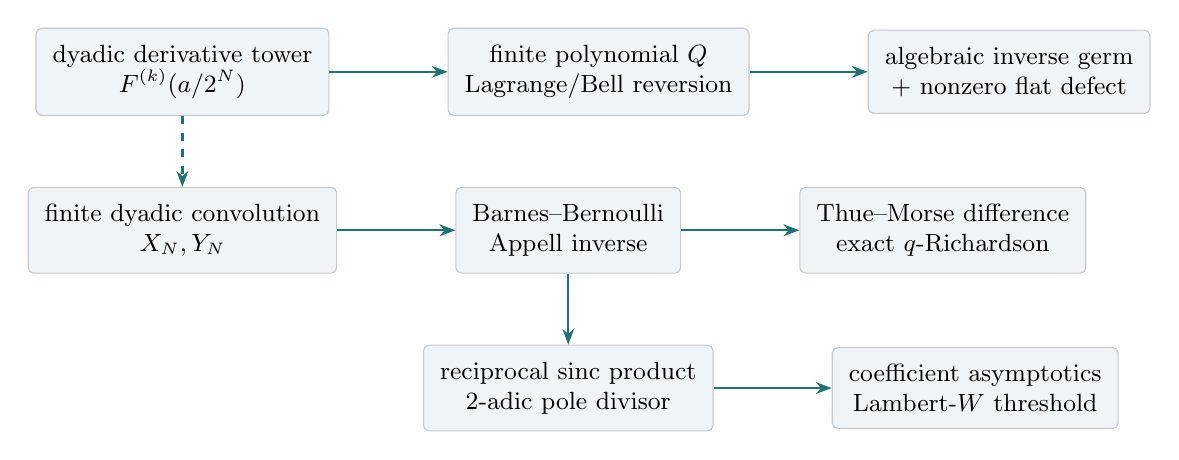
\begin{tikzpicture}[
  node distance=9mm and 15mm,
  every node/.style={draw=RuleGray,rounded corners=2pt,fill=SoftBlue,
                     align=center,inner sep=6pt,font=\small},
  arr/.style={-{Stealth[length=2mm]},thick,draw=Teal}]
  \node (dyadic) {dyadic derivative tower\\$F^{(k)}(a/2^N)$};
  \node (inverse) [right=of dyadic] {finite polynomial $Q$\\Lagrange/Bell reversion};
  \node (flat) [right=of inverse] {algebraic inverse germ\\$+$ nonzero flat defect};
  \node (conv) [below=of dyadic] {finite dyadic convolution\\$X_N,Y_N$};
  \node (barnes) [right=of conv] {Barnes--Bernoulli\\Appell inverse};
  \node (tm) [right=of barnes] {Thue--Morse difference\\exact $q$-Richardson};
  \node (sinc) [below=of barnes] {reciprocal sinc product\\$2$-adic pole divisor};
  \node (lambert) [right=of sinc] {coefficient asymptotics\\Lambert-$W$ threshold};
  \draw[arr] (dyadic)--(inverse);
  \draw[arr] (inverse)--(flat);
  \draw[arr] (conv)--(barnes);
  \draw[arr] (barnes)--(tm);
  \draw[arr] (barnes)--(sinc);
  \draw[arr] (sinc)--(lambert);
  \draw[arr,dashed] (dyadic)--(conv);
\end{tikzpicture}
\end{center}

\section{Established platform and notation}
\label{sec:platform}

\subsection{Fabius, the signed extension, and the Rvachev density}

Let $F:\R\to[0,1]$ be the bounded Fabius function: $F=0$ on $(-\infty,0]$,
$F=1$ on $[1,\infty)$, and on the unit interval
\begin{equation}
 F(1-x)=1-F(x),\qquad F'(x)=2F(2x)\quad(0\le x\le1/2).
 \label{eq:F-basic}
\end{equation}
The Rvachev up-function is the even density supported on $[-1,1]$ for which
\begin{equation}
 F'(x)=2\Up(2x-1),\qquad 0<x<1.
 \label{eq:Fprime-up}
\end{equation}
The repository's signed global extension $\GF$ agrees with $F$ on $[0,1]$ and satisfies
\begin{equation}
 \GF^{(m)}(x)=2^{\binom{m+1}{2}}\GF(2^m x).
 \label{eq:global-derivative}
\end{equation}
At nonnegative integers,
\begin{equation}
 \GF(2r)=0,\qquad \GF(2r+1)=\eps_r,
 \qquad \eps_r=(-1)^{\wt(r)}.
 \label{eq:integer-global}
\end{equation}
Consequently, if $x_0=a/2^N$ is a reduced dyadic point with $a$ odd, then
\begin{equation}
 F^{(m)}(x_0)=0\qquad(m>N).
 \label{eq:dyadic-vanish}
\end{equation}
All derivatives in the finite jet are rational, because the scaled arguments in
\eqref{eq:global-derivative} are dyadic and the repository gives exact rational evaluators there.

\subsection{The two random series}

Let $(U_j)_{j\ge1}$ be independent uniform random variables on $[0,1]$, and let
$(V_j)_{j\ge1}$ be independent uniform random variables on $[-1,1]$.  Put
\begin{equation}
 X=\sum_{j\ge1}2^{-j}U_j,
 \qquad
 Y=\sum_{j\ge1}2^{-j}V_j=2X-1.
 \label{eq:XY-series}
\end{equation}
Then $F$ is the distribution function of $X$ and $\Up$ is the density of $Y$.  Their moment
generating functions are entire:
\begin{align}
 L(t)&=\mathbb E\e^{tX}
 =\prod_{j\ge1}\frac{\e^{t/2^j}-1}{t/2^j},
 \label{eq:L-def}\\
 M(t)&=\mathbb E\e^{tY}
 =\prod_{j\ge1}\frac{\sinh(t/2^j)}{t/2^j}
 =\e^{-t}L(2t).
 \label{eq:M-def}
\end{align}
Self-similarity gives
\begin{equation}
 L(2t)=\frac{\e^t-1}{t}L(t),
 \qquad
 M(2t)=\frac{\sinh t}{t}M(t).
 \label{eq:mgf-refinement}
\end{equation}
On the imaginary axis,
\begin{equation}
 M(2\pi\ii z)=\prod_{k\ge0}\sinc(z/2^k)=:\Phi(z),
 \qquad \sinc u=\frac{\sin(\pi u)}{\pi u}.
 \label{eq:M-Phi}
\end{equation}
Thus the moment problem and the infinite sinc product are two restrictions of the same entire
function.

\subsection{Moments and cumulants}

Write $\kappa_n(X)$ and $\kappa_n(Y)$ for cumulants.  The Bernoulli expansion of
$\log((\e^t-1)/t)$ gives
\begin{align}
 \kappa_1(X)&=\frac12,
 &\kappa_{2r}(X)&=\frac{B_{2r}}{2r(4^r-1)},
 &\kappa_{2r+1}(X)&=0\quad(r\ge1),
 \label{eq:X-cumulants}\\
 \kappa_1(Y)&=0,
 &\kappa_{2r}(Y)&=\frac{2^{2r-1}B_{2r}}{r(4^r-1)},
 &\kappa_{2r+1}(Y)&=0.
 \label{eq:Y-cumulants}
\end{align}
The first centered moments are
\begin{equation}
 m_0=1,
 \quad m_2=\frac19,
 \quad m_4=\frac{19}{675},
 \quad m_6=\frac{583}{59535},
 \quad m_8=\frac{132809}{32531625}.
 \label{eq:Y-moments}
\end{equation}
These established rational sequences will become coefficients in the exact finite-prefix expansion.

\section{Algebraic Taylor shadows of the inverse Fabius function}
\label{sec:inverse-germs}

\subsection{The finite dyadic jet polynomial}

Fix a reduced dyadic point
\begin{equation}
 x_0=\frac{a}{2^N}\in(0,1),\qquad a\ \text{odd},
 \qquad y_0=F(x_0).
 \label{eq:x0-y0}
\end{equation}
Put
\begin{equation}
 f_k=F^{(k)}(x_0)
 =2^{\binom{k+1}{2}}\GF(2^kx_0),
 \qquad
 Q_{x_0}(h)=\sum_{k=1}^{N}\frac{f_k}{k!}h^k.
 \label{eq:Q-dyadic}
\end{equation}
Since $F'(x_0)>0$, the polynomial $Q_{x_0}$ has a nonzero linear term.  The smooth Taylor
remainder
\begin{equation}
 \rho_{x_0}(h):=F(x_0+h)-y_0-Q_{x_0}(h)
 \label{eq:rho-flat}
\end{equation}
is flat at $h=0$: every derivative of $\rho_{x_0}$ vanishes there.  It is not identically zero on any
neighborhood, because $F$ is nowhere analytic in $(0,1)$.

\begin{theorem}[Dyadic algebraic inverse germ; \statusnew]
\label{thm:algebraic-inverse-germ}
Let $\InvF=F^{-1}:(0,1)\to(0,1)$.  There is a unique analytic germ $S_{x_0}$ at $0$ such that
\begin{equation}
 Q_{x_0}(S_{x_0}(z))=z,
 \qquad S_{x_0}(0)=0.
 \label{eq:S-inverse}
\end{equation}
It is an algebraic function over $\Q(z)$.  Moreover
\begin{equation}
 \boxed{
 \InvF(y_0+z)=x_0+S_{x_0}(z)+R_{x_0}(z),
 }
 \label{eq:G-shadow}
\end{equation}
where $R_{x_0}$ is $C^\infty$, flat at $0$, and nonzero in every neighborhood of $0$.
Consequently, the complete Taylor series of $\InvF$ at $y_0$ is convergent and algebraic even
though it does not represent $\InvF$ on any neighborhood.
\end{theorem}

\begin{proof}
The analytic inverse-function theorem applied to the polynomial $Q_{x_0}$ gives the unique analytic
germ $S_{x_0}$.  Since $S_{x_0}$ satisfies the polynomial equation
$Q_{x_0}(w)-z=0$, it is algebraic over $\Q(z)$; rationality of the coefficients of $Q_{x_0}$ follows
from the exact dyadic evaluator.

Let
\[
 H(z)=\InvF(y_0+z)-x_0.
\]
Then
\[
 z=F(x_0+H(z))-y_0=Q_{x_0}(H(z))+\rho_{x_0}(H(z)).
\]
The composite $\rho_{x_0}\circ H$ is flat because $H(0)=0$ and $H'(0)>0$.  Comparing derivatives
recursively in this equation shows that the formal Taylor series of $H$ is the unique formal inverse
of $Q_{x_0}$, hence equals the Taylor series of $S_{x_0}$.  Thus $R_{x_0}=H-S_{x_0}$ is flat.

If $R_{x_0}$ vanished on a neighborhood, then $\InvF$ would agree there with the analytic function
$x_0+S_{x_0}$.  Since $\InvF'(y_0)>0$, the analytic inverse-function theorem would make $F$
analytic at $x_0$, contradicting the nowhere-analyticity theorem.  Therefore $R_{x_0}$ is nonzero in
every neighborhood.
\end{proof}

\begin{resultbox}[The paradox in its sharpest form]
At a dyadic output $y_0=F(a/2^N)$, the inverse Fabius function has a Taylor series with a positive
radius of convergence, and that series is an algebraic function with rational coefficients.  Yet the
sum of the series is not the inverse Fabius function on either side of $y_0$: the discrepancy is a
nontrivial flat germ invisible to every derivative.
\end{resultbox}

\subsection{Lagrange--B\"urmann and Bell formulas}

Factor
\begin{equation}
 Q_{x_0}(u)=u\varphi_{x_0}(u),
 \qquad
 \varphi_{x_0}(0)=f_1>0.
 \label{eq:Q-phi}
\end{equation}
The coefficients of the algebraic inverse are completely explicit.

\begin{theorem}[All inverse derivatives at dyadic outputs; \statusnew]
\label{thm:inverse-derivatives}
For every $m\ge1$,
\begin{equation}
 \boxed{
 \InvF^{(m)}(y_0)
 =(m-1)!\,[u^{m-1}]\,\varphi_{x_0}(u)^{-m}.
 }
 \label{eq:Lagrange-inverse-derivative}
\end{equation}
Equivalently, if $g_m=\InvF^{(m)}(y_0)$ and $B_{m,k}$ denotes the partial exponential Bell
polynomial, then
\begin{align}
 g_1&=\frac1{f_1},
 \label{eq:g1}\\
 g_m&=-\frac1{f_1}
 \sum_{k=2}^{\min(m,N)}f_k
 B_{m,k}(g_1,g_2,\ldots,g_{m-k+1})
 \qquad(m\ge2).
 \label{eq:Bell-inverse-recurrence}
\end{align}
In particular, every $\InvF^{(m)}(y_0)$ is rational.
\end{theorem}

\begin{proof}
The Lagrange--B\"urmann formula for the inverse of $z=u\varphi_{x_0}(u)$ gives
\[
 [z^m]S_{x_0}(z)=\frac1m[u^{m-1}]\varphi_{x_0}(u)^{-m}.
\]
Multiplication by $m!$ proves \eqref{eq:Lagrange-inverse-derivative}.  For the Bell recurrence,
differentiate $F(\InvF(y))=y$ $m$ times at $y=y_0$.  Fa\`a di Bruno gives
\[
 \sum_{k=1}^{m} f_k B_{m,k}(g_1,\ldots,g_{m-k+1})=0\qquad(m\ge2).
\]
Since $B_{m,1}=g_m$, solving for the newest derivative gives
\eqref{eq:Bell-inverse-recurrence}.  All inputs are rational.
\end{proof}

\begin{remark}
The formulas use two different Bell-polynomial roles in the same theory.  Partial Bell polynomials
invert composition in \eqref{eq:Bell-inverse-recurrence}; complete Bell polynomials will invert a
moment generating function in \cref{sec:appell}.  The two appearances are not cosmetic variants:
one organizes set partitions by the number of blocks, while the other sums over all block counts.
\end{remark}

\subsection{The midpoint: a linear Taylor shadow}

At $x_0=1/2$ one has $y_0=1/2$, $F'(1/2)=2$, and all higher derivatives vanish.  Hence
\begin{equation}
 Q_{1/2}(h)=2h,
 \qquad
 S_{1/2}(z)=\frac z2.
 \label{eq:midpoint-shadow}
\end{equation}
Thus
\begin{equation}
 \InvF(1/2+z)=\frac12+\frac z2+R_{1/2}(z),
 \label{eq:midpoint-flat}
\end{equation}
where $R_{1/2}$ is a nonzero flat odd germ.  Every derivative of $\InvF$ at $1/2$ beyond the first is
zero, but $\InvF$ is not linear on any neighborhood.

\subsection{The quarter point: Catalan numbers exactly}

The first nontrivial case is unexpectedly rigid.

\begin{theorem}[Catalan inverse jet at $F(1/4)$; \statusnew]
\label{thm:Catalan-quarter}
The exact value and derivative jet at $x_0=1/4$ are
\begin{equation}
 F(1/4)=\frac5{72},
 \qquad F'(1/4)=1,
 \qquad F''(1/4)=8,
 \qquad F^{(m)}(1/4)=0\ (m\ge3).
 \label{eq:quarter-jet}
\end{equation}
Therefore
\begin{equation}
 Q_{1/4}(h)=h+4h^2,
 \qquad
 S_{1/4}(z)=\frac{\sqrt{1+16z}-1}{8}.
 \label{eq:quarter-shadow}
\end{equation}
For every $m\ge1$,
\begin{equation}
 \boxed{
 \InvF^{(m)}(5/72)
 =m!(-1)^{m-1}4^{m-1}C_{m-1},
 \qquad C_r=\frac1{r+1}\binom{2r}{r}.
 }
 \label{eq:Catalan-derivatives}
\end{equation}
The corresponding large-order law is
\begin{equation}
 \left|\InvF^{(m)}(5/72)\right|
 \sim \frac{m!\,16^{m-1}}{\sqrt\pi\,(m-1)^{3/2}}.
 \label{eq:Catalan-asymptotic}
\end{equation}
\end{theorem}

\begin{proof}
The value $F(1/4)=5/72$ is part of the repository's exact dyadic table.  From
\eqref{eq:global-derivative},
\[
 F'(1/4)=2F(1/2)=1,
 \qquad
 F''(1/4)=8\GF(1)=8,
\]
and \eqref{eq:dyadic-vanish} removes all higher derivatives.  Solving
$z=h+4h^2$ for the branch with $h(0)=0$ gives \eqref{eq:quarter-shadow}.  The classical Catalan
generating function
\[
 \frac{\sqrt{1+16z}-1}{8}
 =\sum_{m\ge1}(-1)^{m-1}4^{m-1}C_{m-1}z^m
\]
proves \eqref{eq:Catalan-derivatives}.  Stirling's estimate
$C_r\sim4^r/(\sqrt\pi r^{3/2})$ proves \eqref{eq:Catalan-asymptotic}.
\end{proof}

\begin{example}[The first derivatives]
\begin{align*}
 \InvF'(5/72)&=1,
 & \InvF''(5/72)&=-8,
 & \InvF^{(3)}(5/72)&=192,\\
 \InvF^{(4)}(5/72)&=-7680,
 & \InvF^{(5)}(5/72)&=430080.
\end{align*}
These rapidly growing derivatives belong to the algebraic square-root shadow.  They do not imply
analyticity of $\InvF$: the actual function differs by a flat germ.
\end{example}

\subsection{The eighth point: a cubic algebraic shadow}

At $x_0=1/8$, the exact value is $F(1/8)=1/288$ and
\begin{equation}
 F'(1/8)=\frac5{36},
 \qquad F''(1/8)=4,
 \qquad F^{(3)}(1/8)=64.
 \label{eq:eighth-jet}
\end{equation}
Thus the inverse Taylor series at $1/288$ is the branch at the origin of
\begin{equation}
 z=\frac5{36}h+2h^2+\frac{32}{3}h^3.
 \label{eq:eighth-cubic}
\end{equation}
This gives an explicit cubic algebraic function and, through
\eqref{eq:Lagrange-inverse-derivative}, a one-line coefficient formula
\begin{equation}
 \InvF^{(m)}(1/288)
 =(m-1)![u^{m-1}]
 \left(\frac5{36}+2u+\frac{32}{3}u^2\right)^{-m}.
 \label{eq:eighth-coeff}
\end{equation}
The quarter point is therefore not an isolated curiosity: every dyadic input produces a finite
algebraic shadow, with degree equal to the reduced denominator exponent.

\subsection{A general singularity program for inverse derivatives}

The nearest singularities of $S_{x_0}$ occur among the critical values
\begin{equation}
 z_c=Q_{x_0}(u_c),
 \qquad Q_{x_0}'(u_c)=0.
 \label{eq:critical-values}
\end{equation}
When the nearest critical point is simple, $S_{x_0}$ has a square-root singularity and its Taylor
coefficients have the universal $m^{-3/2}$ factor seen in \eqref{eq:Catalan-asymptotic}.  Multiple
critical points lead to other Puiseux exponents.  Since $Q_{x_0}$ is exactly computable over $\Q$,
this converts the high-order inverse-derivative problem at every dyadic output into finite algebraic
geometry.

\begin{frontierbox}[Frontier problem: dyadic inverse singularity atlas]
For each reduced dyadic $a/2^N$, classify the critical values of $Q_{a/2^N}$, determine which one
sets the convergence radius of the inverse Taylor shadow, and describe the Galois and $2$-adic
structure of the resulting Puiseux constants.  The case $N=2$ is Catalan; the case $N=3$ is cubic;
already $N=4$ should reveal whether a stable binary pattern exists.
\end{frontierbox}

\section{Kabaya--Iri polynomials and the Rvachev Appell inverse}
\label{sec:appell}

\subsection{The external precursor and the normalization used here}

Lee's scaling-polynomial construction associates to a compactly supported probability density
$\phi$ the Appell sequence generated by $\e^{xt}/\widehat\phi(\ii t)$ and proves its biorthogonality
to the distributional derivatives of $\phi$.  For the up-function, these are the Kabaya--Iri
polynomials.  In the Fabius normalization used in this report, it is convenient to distinguish the
uncentered law $X\in[0,1]$ from the centered law $Y=2X-1\in[-1,1]$.

\begin{definition}[Kabaya--Iri and centered Rvachev--Appell polynomials]
\label{def:Appell-polys}
Define $P_n,A_n\in\Q[x]$ by
\begin{align}
 \frac{\e^{xt}}{L(t)}
 &=\sum_{n\ge0}P_n(x)\frac{t^n}{n!},
 \label{eq:P-generating}\\
 \frac{\e^{xt}}{M(t)}
 &=\sum_{n\ge0}A_n(x)\frac{t^n}{n!}.
 \label{eq:A-generating}
\end{align}
\end{definition}

The affine change $M(t)=\e^{-t}L(2t)$ gives
\begin{equation}
 \boxed{
 A_n(x)=2^nP_n\!\left(\frac{x+1}{2}\right),
 \qquad
 P_n(x)=2^{-n}A_n(2x-1).
 }
 \label{eq:A-P-affine}
\end{equation}
Thus the sequence $P_n$ is the known Kabaya--Iri sequence, while $A_n$ is its symmetric Rvachev
normalization.  The centering eliminates every odd cumulant and makes the pole analysis in
\cref{sec:poles} transparent.

\subsection{Appell, mean-value, and biorthogonality identities}

\begin{proposition}[Classical Appell package; \statuslit]
\label{prop:Appell-package}
For $n\ge1$,
\begin{align}
 P_n'(x)&=nP_{n-1}(x),
 &A_n'(x)&=nA_{n-1}(x),
 \label{eq:Appell-derivative}\\
 P_n(x+y)&=\sum_{k=0}^n\binom nkP_k(x)y^{n-k},
 &A_n(x+y)&=\sum_{k=0}^n\binom nkA_k(x)y^{n-k}.
 \label{eq:Appell-translation}
\end{align}
The polynomial averaging operators are inverted exactly:
\begin{equation}
 \boxed{
 \mathbb E\,P_n(x+X)=x^n,
 \qquad
 \mathbb E\,A_n(x+Y)=x^n.
 }
 \label{eq:mean-value-inversion}
\end{equation}
If $f_X=F'$ is the density of $X$, then in the distributional sense
\begin{equation}
 \left\langle(-1)^r f_X^{(r)},\frac{P_n}{n!}\right\rangle=\delta_{rn}.
 \label{eq:P-biorthogonal}
\end{equation}
Equivalently, for the centered density $\Up$,
\begin{equation}
 \int_{-1}^{1}(-1)^r\Up^{(r)}(x)\frac{A_n(x)}{n!}\,\dd x
 =\delta_{rn}.
 \label{eq:A-biorthogonal}
\end{equation}
\end{proposition}

\begin{proof}
Differentiate the generating functions with respect to $x$ to obtain
\eqref{eq:Appell-derivative}; multiply by $\e^{yt}$ to obtain
\eqref{eq:Appell-translation}.  For the mean-value identities,
\[
 \mathbb E\sum_{n\ge0}P_n(x+X)\frac{t^n}{n!}
 =\mathbb E\frac{\e^{(x+X)t}}{L(t)}=\e^{xt},
\]
and similarly for $A_n$.  The biorthogonality is Lee's general compactly supported
distribution identity specialized to $f_X$ and transported affinely to $\Up$.  It can also be checked
directly by repeated integration by parts and \eqref{eq:mean-value-inversion}.
\end{proof}

\begin{remark}
Equation \eqref{eq:mean-value-inversion} is an exact polynomial deconvolution formula.  The operator
$\mathcal T_Y:p\mapsto\mathbb E p(\,\cdot+Y)$ is triangular on $\Q[x]$ with ones on its diagonal;
$A_n=\mathcal T_Y^{-1}x^n$.  This is the linear inverse problem announced in
\cref{sec:scope}.
\end{remark}

\subsection{Bell reconstruction from Bernoulli cumulants}

Set
\begin{equation}
 \alpha_n=A_n(0),
 \qquad
 \frac1{M(t)}=\sum_{n\ge0}\alpha_n\frac{t^n}{n!}.
 \label{eq:alpha-def}
\end{equation}
Symmetry gives $\alpha_{2r+1}=0$.  If $\Bell_n$ denotes the complete exponential Bell polynomial,
then \eqref{eq:Y-cumulants} yields
\begin{equation}
 \boxed{
 \alpha_n=\Bell_n\bigl(-\kappa_1(Y),-\kappa_2(Y),\ldots,-\kappa_n(Y)\bigr).
 }
 \label{eq:alpha-Bell}
\end{equation}
Equivalently,
\begin{equation}
 \alpha_0=1,
 \qquad
 \alpha_n=-\sum_{j=1}^n\binom{n-1}{j-1}\kappa_j(Y)\alpha_{n-j}.
 \label{eq:alpha-recurrence}
\end{equation}
The first constants are
\begin{equation}
 \alpha_0=1,
 \quad \alpha_2=-\frac19,
 \quad \alpha_4=\frac{31}{675},
 \quad \alpha_6=-\frac{2347}{59535},
 \quad \alpha_8=\frac{1904369}{32531625}.
 \label{eq:alpha-first}
\end{equation}
The Appell translation law then gives
\begin{equation}
 A_n(x)=\sum_{k=0}^n\binom nk\alpha_{n-k}x^k.
 \label{eq:A-from-alpha}
\end{equation}
For reference,
\begin{equation}
\begin{aligned}
 A_0(x)&=1,\\
 A_1(x)&=x,\\
 A_2(x)&=x^2-\frac19,\\
 A_3(x)&=x^3-\frac13x,\\
 A_4(x)&=x^4-\frac23x^2+\frac{31}{675},\\
 A_5(x)&=x^5-\frac{10}{9}x^3+\frac{31}{135}x,\\
 A_6(x)&=x^6-\frac53x^4+\frac{31}{45}x^2-\frac{2347}{59535}.
\end{aligned}
\label{eq:A-first-polys}
\end{equation}
Using \eqref{eq:A-P-affine}, the first uncentered polynomials are
\begin{equation}
\begin{aligned}
 P_0(x)&=1,\\
 P_1(x)&=x-\frac12,\\
 P_2(x)&=x^2-x+\frac29,\\
 P_3(x)&=x^3-\frac32x^2+\frac23x-\frac1{12},\\
 P_4(x)&=x^4-2x^3+\frac43x^2-\frac13x+\frac{16}{675},\\
 P_5(x)&=x^5-\frac52x^4+\frac{20}{9}x^3-\frac56x^2+\frac{16}{135}x-\frac1{270}.
\end{aligned}
\label{eq:P-first-polys}
\end{equation}
These agree with Lee's displayed Kabaya--Iri list through degree five.

\subsection{Bernoulli refinement recurrences}

The self-similarity identities \eqref{eq:mgf-refinement} become polynomial recurrences when the
reciprocal generating functions are compared.

\begin{proposition}[Bernoulli refinement of the Appell sequences]
\label{prop:Bernoulli-refinement}
Let $B_k$ be defined by $t/(\e^t-1)=\sum B_kt^k/k!$, and let
$c_{2r}=2(1-2^{2r-1})B_{2r}$ be the exponential coefficients of
$t/\sinh t$.  Then
\begin{align}
 2^nP_n(x)
 &=\sum_{k=0}^n\binom nkB_kP_{n-k}(2x),
 \label{eq:P-Bernoulli-refinement}\\
 2^nA_n(x)
 &=\sum_{r=0}^{\lfloor n/2\rfloor}
   \binom n{2r}c_{2r}A_{n-2r}(2x).
 \label{eq:A-Bernoulli-refinement}
\end{align}
\end{proposition}

\begin{proof}
Substitute \eqref{eq:mgf-refinement} into the defining generating functions:
\begin{align*}
 \frac{\e^{2xt}}{L(2t)}
 &=\frac{t}{\e^t-1}\frac{\e^{2xt}}{L(t)},\\
 \frac{\e^{2xt}}{M(2t)}
 &=\frac{t}{\sinh t}\frac{\e^{2xt}}{M(t)}.
\end{align*}
Coefficient comparison gives the two formulas.
\end{proof}

\begin{remark}
The repository's Bernoulli recurrences usually govern moments, reciprocal sine products, or saddle
coefficients.  Here the same Bernoulli numbers govern a polynomial eigenbasis for the adjoint
Rvachev averaging operator.  The recurrence is a direct algebraic shadow of dyadic refinement.
\end{remark}

\subsection{A dyadic logistic dual}

The complete Bell signs in \eqref{eq:alpha-first} admit a probabilistic explanation that appears not
to have been recorded for the Rvachev law.

Let $\Lambda$ be a standard logistic random variable with density
\begin{equation}
 \ell(x)=\frac{\e^{-x}}{(1+\e^{-x})^2}.
 \label{eq:logistic-density}
\end{equation}
The beta integral gives
\begin{equation}
 \mathbb E\e^{\ii t\Lambda}
 =\Gamma(1+\ii t)\Gamma(1-\ii t)
 =\frac{\pi t}{\sinh(\pi t)}.
 \label{eq:logistic-cf}
\end{equation}
Let $(\Lambda_j)_{j\ge1}$ be independent copies and define
\begin{equation}
 Z=\sum_{j\ge1}\frac{\Lambda_j}{\pi2^j}.
 \label{eq:Z-logistic}
\end{equation}
The series converges in $L^2$ and almost surely.

\begin{theorem}[Logistic dual of the Rvachev law; \statusnew]
\label{thm:logistic-dual}
For real $t$,
\begin{equation}
 \boxed{
 \mathbb E\e^{\ii tZ}
 =\prod_{j\ge1}\frac{t/2^j}{\sinh(t/2^j)}
 =\frac1{M(t)}.
 }
 \label{eq:Z-cf}
\end{equation}
Consequently, as polynomial identities,
\begin{align}
 A_n(x)&=\mathbb E\,(x+\ii Z)^n,
 \label{eq:A-logistic-moment}\\
 P_n(x)&=\mathbb E\left(x-\frac12+\frac{\ii Z}{2}\right)^n.
 \label{eq:P-logistic-moment}
\end{align}
In particular,
\begin{equation}
 \boxed{
 \alpha_{2m}=(-1)^m\mathbb E Z^{2m},
 \qquad (-1)^m\alpha_{2m}>0.
 }
 \label{eq:alpha-sign}
\end{equation}
\end{theorem}

\begin{proof}
Independence and \eqref{eq:logistic-cf} give
\[
 \mathbb E\e^{\ii tZ}
 =\prod_{j\ge1}
 \frac{t/2^j}{\sinh(t/2^j)}=\frac1{M(t)}.
\]
The product converges locally uniformly on the real axis because the logarithm of its $j$th factor
is $\BigO(4^{-j}t^2)$.  Multiplying by $\e^{xt}$ and comparing the Taylor expansion at $0$ proves
\eqref{eq:A-logistic-moment}.  The affine identity \eqref{eq:A-P-affine} gives
\eqref{eq:P-logistic-moment}.  Setting $x=0$ and using symmetry of $Z$ proves
\eqref{eq:alpha-sign}.
\end{proof}

\begin{resultbox}[A duality of compact and noncompact laws]
The Rvachev variable $Y$ is compactly supported and has moment generating function $M$.  Its
polynomial deconvolution sequence is represented by imaginary moments of the noncompact variable
$Z$, an infinite dyadic sum of logistic variables, whose characteristic function is $M^{-1}$.
Thus the reciprocal sinc product is not merely a formal series: on the real axis it is itself a
positive-definite characteristic function.
\end{resultbox}

\subsection{Operator interpretation}

Let $D=\dd/\dd x$.  On polynomials,
\begin{equation}
 \mathcal T_Y=\mathbb E\e^{YD}=M(D),
 \qquad
 \mathcal T_Y^{-1}=M(D)^{-1}=\mathbb E\e^{\ii ZD}.
 \label{eq:operator-deconvolution}
\end{equation}
Therefore
\begin{equation}
 A_n=M(D)^{-1}x^n.
 \label{eq:A-operator}
\end{equation}
This identity packages the mean-value theorem, the logistic dual, and the Appell derivative rule in
one line.  It also prepares the finite Barnes and Thue--Morse difference calculus: replacing $M$ by
a finite product replaces the infinite-order differential operator by a finite product of Bernoulli
operators.

\section{Finite dyadic prefixes as Barnes--Bernoulli polynomials}
\label{sec:barnes}

\subsection{Finite random sums and finite Appell inverses}

For $N\ge1$, define the convolution prefixes
\begin{equation}
 X_N=\sum_{j=1}^{N}2^{-j}U_j,
 \qquad
 Y_N=\sum_{j=1}^{N}2^{-j}V_j,
 \label{eq:finite-XY}
\end{equation}
with moment generating functions
\begin{align}
 L_N(t)&=\prod_{j=1}^{N}\frac{\e^{t/2^j}-1}{t/2^j},
 \label{eq:LN}\\
 M_N(t)&=\prod_{j=1}^{N}\frac{\sinh(t/2^j)}{t/2^j}.
 \label{eq:MN}
\end{align}
Define finite-prefix Appell polynomials by
\begin{align}
 \frac{\e^{xt}}{L_N(t)}
 &=\sum_{n\ge0}P_n^{[N]}(x)\frac{t^n}{n!},
 \label{eq:PN-generating}\\
 \frac{\e^{xt}}{M_N(t)}
 &=\sum_{n\ge0}A_n^{[N]}(x)\frac{t^n}{n!}.
 \label{eq:AN-generating}
\end{align}
They satisfy the exact finite mean-value identities
\begin{equation}
 \mathbb E P_n^{[N]}(x+X_N)=x^n,
 \qquad
 \mathbb E A_n^{[N]}(x+Y_N)=x^n.
 \label{eq:finite-mean-value}
\end{equation}
Because $X_N$ and $Y_N$ are finite convolutions of boxes, these polynomials are the exact
polynomial duals of the spline approximants developed elsewhere in the repository.

\subsection{Normalized Barnes multiple Bernoulli polynomials}

For nonzero periods $b_1,\ldots,b_N$, define the normalized Barnes multiple Bernoulli polynomials
$\mathfrak B_n^{(N)}$ by
\begin{equation}
 \e^{xt}\prod_{j=1}^{N}\frac{b_jt}{\e^{b_jt}-1}
 =\sum_{n\ge0}
 \mathfrak B_n^{(N)}(x\mid b_1,\ldots,b_N)\frac{t^n}{n!}.
 \label{eq:Barnes-def}
\end{equation}
This normalization has leading coefficient one and reduces to the ordinary Bernoulli polynomial
when $N=1$ and $b_1=1$.

\begin{theorem}[Dyadic Barnes identification; \statusnew]
\label{thm:Barnes-identification}
For every $N,n\ge0$,
\begin{equation}
 \boxed{
 P_n^{[N]}(x)
 =\mathfrak B_n^{(N)}
 \left(x\mid 2^{-1},2^{-2},\ldots,2^{-N}\right).
 }
 \label{eq:P-Barnes}
\end{equation}
Let
\begin{equation}
 s_N=1-2^{-N},
 \qquad
 (a_1,\ldots,a_N)=(1,1/2,\ldots,2^{1-N}).
 \label{eq:a-sN}
\end{equation}
Then
\begin{equation}
 \boxed{
 A_n^{[N]}(x)
 =\mathfrak B_n^{(N)}
 \left(x+s_N\mid1,\frac12,\ldots,2^{1-N}\right).
 }
 \label{eq:A-Barnes}
\end{equation}
\end{theorem}

\begin{proof}
Equation \eqref{eq:P-Barnes} is immediate by comparing
\eqref{eq:PN-generating} with \eqref{eq:Barnes-def}.  For the centered product, write
\[
 \frac{\sinh(a_jt/2)}{a_jt/2}
 =\e^{-a_jt/2}\frac{\e^{a_jt}-1}{a_jt}.
\]
Since $\frac12\sum_{j=1}^{N}a_j=s_N$, one has
\[
 \frac{\e^{xt}}{M_N(t)}
 =\e^{(x+s_N)t}\prod_{j=1}^{N}\frac{a_jt}{\e^{a_jt}-1},
\]
which is \eqref{eq:A-Barnes}.
\end{proof}

\begin{remark}
The period vectors are geometric rather than repeated.  This is a Barnes analogue of the
repository's ubiquitous $q=1/2$ geometry: each new convolution scale appends one period to the
multiple Bernoulli polynomial.  The infinite Kabaya--Iri sequence is therefore a geometric-period
limit of a Barnes tower.
\end{remark}

\subsection{A complete Thue--Morse difference operator}

For a step $h$, write $E_h=\e^{hD}$ for translation: $(E_hp)(x)=p(x+h)$.  The complete binary
signed difference operator is
\begin{equation}
 \Delta_N^{\mathrm{TM}}(b_1,\ldots,b_N)
 :=\prod_{j=1}^{N}(1-E_{b_j}).
 \label{eq:TM-operator}
\end{equation}
Expanding the product assigns a sign $(-1)^{|J|}$ to each subset $J$.  With geometric steps, subset
sums are binary integers and the signs are precisely Thue--Morse.

\begin{theorem}[Uncentered Thue--Morse--Barnes collapse; \statusnew]
\label{thm:TM-uncentered}
Let $\eps_k=(-1)^{\wt(k)}$.  For every $N\ge1$ and $n\ge0$,
\begin{equation}
 \boxed{
 \sum_{k=0}^{2^N-1}\eps_k
 P_n^{[N]}\!\left(x+\frac{k}{2^N}\right)
 =(-1)^N2^{-N(N+1)/2}\fall nN\,x^{n-N},
 }
 \label{eq:TM-P-collapse}
\end{equation}
where the right side is interpreted as zero when $n<N$.
\end{theorem}

\begin{proof}
Multiply the generating function \eqref{eq:PN-generating} by the complete signed exponential sum:
\begin{align*}
 \sum_{k=0}^{2^N-1}\eps_k
 \frac{\e^{(x+k/2^N)t}}{L_N(t)}
 &=\frac{\e^{xt}}{L_N(t)}
   \prod_{j=1}^{N}(1-\e^{t/2^j})\\
 &=(-1)^N\e^{xt}t^N\prod_{j=1}^{N}2^{-j}\\
 &=(-1)^N2^{-N(N+1)/2}t^N\e^{xt}.
\end{align*}
The coefficient of $t^n/n!$ is the stated monomial.
\end{proof}

\begin{corollary}[Prouhet cancellation with a canonical correction]
\label{cor:Prouhet-canonical}
For $n<N$, the complete Thue--Morse sum in \eqref{eq:TM-P-collapse} vanishes.  For $n=N$, it is the
constant
\begin{equation}
 (-1)^NN!\,2^{-N(N+1)/2}.
 \label{eq:TM-first-nonzero}
\end{equation}
For $n>N$, it is exactly the monomial response of an $N$th finite difference.  Thus the finite
Kabaya--Iri polynomial is a canonical polynomial on which the Prouhet cancellation defect is
completely diagonalized.
\end{corollary}

The centered form is sign-cleaner because the support is arranged symmetrically.

\begin{theorem}[Centered Thue--Morse--Rvachev collapse; \statusnew]
\label{thm:TM-centered}
With $s_N=1-2^{-N}$, for every $N\ge1$ and $n\ge0$,
\begin{equation}
 \boxed{
 \sum_{k=0}^{2^N-1}\eps_k
 A_n^{[N]}\!\left(x+s_N-\frac{k}{2^{N-1}}\right)
 =2^{-N(N-1)/2}\fall nN\,x^{n-N}.
 }
 \label{eq:TM-A-collapse}
\end{equation}
\end{theorem}

\begin{proof}
The binary subset sums of the period vector
$(1,1/2,\ldots,2^{1-N})$ are $k/2^{N-1}$.  Hence
\begin{align*}
 &\sum_{k=0}^{2^N-1}\eps_k
 \frac{\e^{(x+s_N-k/2^{N-1})t}}{M_N(t)}\\
 &\qquad=
 \frac{\e^{(x+s_N)t}}{M_N(t)}
 \prod_{j=1}^{N}(1-\e^{-a_jt}).
\end{align*}
Now
\[
 \prod_{j=1}^{N}(1-\e^{-a_jt})
 =\e^{-2s_Nt}\prod_{j=1}^{N}(\e^{a_jt}-1),
\]
while
\[
 M_N(t)^{-1}=\e^{s_Nt}\prod_{j=1}^{N}\frac{a_jt}{\e^{a_jt}-1}.
\]
All exponentials cancel, leaving
$\e^{xt}t^N\prod_ja_j=2^{-N(N-1)/2}t^N\e^{xt}$.  Coefficient comparison proves the theorem.
\end{proof}

\begin{example}[The first genuinely centered identity]
For $N=2$,
\begin{equation}
 A_4^{[2]}(x)=x^4-\frac58x^2+\frac{53}{1280}.
 \label{eq:A4N2}
\end{equation}
The four-point Thue--Morse difference is
\begin{align}
 &A_4^{[2]}(x+3/4)-A_4^{[2]}(x+1/4)
 -A_4^{[2]}(x-1/4)+A_4^{[2]}(x-3/4)
 \notag\\
 &\hspace{5cm}=6x^2.
 \label{eq:A4N2-example}
\end{align}
The constants and lower even powers disappear exactly, not asymptotically.
\end{example}

\subsection{A q-binomial form of the difference operator}

The Thue--Morse block polynomial
\begin{equation}
 T_N(z)=\sum_{k=0}^{2^N-1}\eps_kz^k
 =\prod_{r=0}^{N-1}(1-z^{2^r})
 \label{eq:TN}
\end{equation}
encodes the same operation as \eqref{eq:TM-operator}.  The collapse theorems can therefore be read
in three interchangeable languages:
\begin{equation}
 \text{binary subset signs}
 \longleftrightarrow
 \text{Thue--Morse block polynomial}
 \longleftrightarrow
 \text{product of Barnes difference factors}.
 \label{eq:three-languages}
\end{equation}
This is a new bridge between the formula atlas and the finite convolution/Barnes hierarchy.  It also
suggests a higher-rank extension: replace the simple product of differences by the Pascal-weighted
multiplicities of the repository's rank-$r$ Rvachev hierarchy, which should produce multiple
Thue--Morse--Barnes operators with repeated geometric periods.

\section{Exact finite-prefix expansions and \texorpdfstring{$q$}{q}-Richardson recovery}
\label{sec:richardson}

\subsection{Tail self-similarity is polynomial in the truncation scale}

Let $X',Y'$ be independent copies of $X,Y$, independent of the first $N$ summands.  Splitting the
random series after level $N$ gives the exact distributional identities
\begin{equation}
 X\overset{d}=X_N+2^{-N}X',
 \qquad
 Y\overset{d}=Y_N+2^{-N}Y'.
 \label{eq:tail-self-similarity}
\end{equation}
Hence
\begin{equation}
 L(t)=L_N(t)L(2^{-N}t),
 \qquad
 M(t)=M_N(t)M(2^{-N}t).
 \label{eq:finite-infinite-mgf}
\end{equation}
Write $\mu_r=\mathbb EX^r$ and $m_{2r}=\mathbb EY^{2r}$.

\begin{theorem}[Exact finite-prefix expansion; \statusnew]
\label{thm:finite-prefix-expansion}
For every $N,n\ge0$,
\begin{equation}
 \boxed{
 P_n^{[N]}(x)
 =\sum_{r=0}^{n}\binom nr\mu_r\,2^{-Nr}P_{n-r}(x).
 }
 \label{eq:P-prefix-expansion}
\end{equation}
For the centered sequence,
\begin{equation}
 \boxed{
 A_n^{[N]}(x)
 =\sum_{r=0}^{\lfloor n/2\rfloor}
 \binom n{2r}m_{2r}\,4^{-Nr}A_{n-2r}(x).
 }
 \label{eq:A-prefix-expansion}
\end{equation}
Thus $P_n^{[N]}(x)$ is exactly a polynomial of degree $n$ in $2^{-N}$, while
$A_n^{[N]}(x)$ is exactly a polynomial of degree $\lfloor n/2\rfloor$ in $4^{-N}$.
\end{theorem}

\begin{proof}
From \eqref{eq:finite-infinite-mgf},
\begin{align*}
 \frac{\e^{xt}}{L_N(t)}
 &=L(2^{-N}t)\frac{\e^{xt}}{L(t)},\\
 \frac{\e^{xt}}{M_N(t)}
 &=M(2^{-N}t)\frac{\e^{xt}}{M(t)}.
\end{align*}
Expand the first extra factor in moments and compare exponential generating coefficients.  In the
centered case all odd moments vanish, so only powers $2^{-2Nr}=4^{-Nr}$ survive.
\end{proof}

\begin{remark}
Earlier extrapolation results in the repository accelerate an infinite sinc product or extract
periodic endpoint coefficients from asymptotic series.  Here there is no asymptotic remainder at
all.  For each fixed polynomial degree, the dependence on the prefix depth is finite and algebraic.
Richardson extrapolation becomes exact interpolation at the missing node $0$.
\end{remark}

\subsection{Geometric Lagrange weights}

Fix $0<q<1$ and an order $p\ge0$.  The Lagrange weights that evaluate a degree-$p$ polynomial at
zero from its values at $1,q,\ldots,q^p$ are
\begin{equation}
 w_{p,j}(q)
 =\prod_{\substack{0\le\ell\le p\\\ell\ne j}}
 \frac{-q^\ell}{q^j-q^\ell}
 \qquad(0\le j\le p).
 \label{eq:w-Lagrange}
\end{equation}
They have the Gaussian-binomial form
\begin{equation}
 \boxed{
 w_{p,j}(q)
 =\frac{(-1)^{p-j}q^{\binom{p-j+1}{2}}}
 {(q;q)_j(q;q)_{p-j}}
 =\frac{(-1)^{p-j}q^{\binom{p-j+1}{2}}}{(q;q)_p}
 \qbinom pj q.
 }
 \label{eq:w-qbinomial}
\end{equation}
The interpolation moments are
\begin{equation}
 \sum_{j=0}^{p}w_{p,j}(q)q^{jr}
 =\begin{cases}
 1,&r=0,\\
 0,&1\le r\le p.
 \end{cases}
 \label{eq:w-annihilation}
\end{equation}

\begin{theorem}[Exact $q$-Richardson recovery; \statusnew]
\label{thm:exact-recovery}
For every $n,N\ge0$,
\begin{equation}
 \boxed{
 P_n(x)=\sum_{j=0}^{n}w_{n,j}(1/2)P_n^{[N+j]}(x).
 }
 \label{eq:P-exact-recovery}
\end{equation}
Let $d=\lfloor n/2\rfloor$.  Then
\begin{equation}
 \boxed{
 A_n(x)=\sum_{j=0}^{d}w_{d,j}(1/4)A_n^{[N+j]}(x).
 }
 \label{eq:A-exact-recovery}
\end{equation}
Both identities hold for every starting depth $N$, not merely in a limit.
\end{theorem}

\begin{proof}
In \eqref{eq:P-prefix-expansion}, set $z=2^{-N}$.  The right side is a polynomial in $z$ of degree
at most $n$, and its value at $z=0$ is $P_n(x)$.  The values at depths $N+j$ are the values at
$zq^j$ with $q=1/2$.  Lagrange interpolation at zero is scale-invariant, so the weights are
$w_{n,j}(1/2)$.  The centered proof is identical with $z=4^{-N}$, degree $d$, and $q=1/4$.
\end{proof}

\begin{resultbox}[Richardson without an error term]
For fixed degree $n$, the infinite Rvachev-Appell polynomial is a finite linear combination of the
Barnes polynomials associated with any $d+1$ consecutive dyadic convolution prefixes.  The outer
weights are Gaussian $q$-binomial coefficients.  The construction therefore joins four structures
that the repository previously treated in separate contexts:
\[
 \text{finite splines}
 \longleftrightarrow
 \text{Barnes periods}
 \longleftrightarrow
 \text{$q$-Lagrange interpolation}
 \longleftrightarrow
 \text{the infinite Rvachev law}.
\]
\end{resultbox}

\subsection{Residual moments beyond the exact degree}

For later perturbations it is useful to know every nonvanishing geometric moment of the weights.
Let $h_r$ be the complete homogeneous symmetric polynomial.  For $r\ge p+1$,
\begin{equation}
 \boxed{
 \sum_{j=0}^{p}w_{p,j}(q)q^{jr}
 =(-1)^pq^{\binom{p+1}{2}}
 h_{r-p-1}(1,q,\ldots,q^p).
 }
 \label{eq:w-residual}
\end{equation}
Indeed, the generating function of the left side is
\begin{align*}
 \sum_{r\ge0}\left(\sum_{j=0}^{p}w_{p,j}(q)q^{jr}\right)z^r
 &=\sum_{j=0}^{p}\frac{w_{p,j}(q)}{1-q^jz}\\
 &=1+(-1)^pq^{\binom{p+1}{2}}
 \frac{z^{p+1}}{\prod_{j=0}^{p}(1-q^jz)}.
\end{align*}
This identity is the exact analogue of the transformed-moment formulas used in classical
Richardson error analysis.  Here it also quantifies what happens when a numerical or symbolic
approximation replaces the exact prefix polynomial.

\subsection{Worked centered recovery in degree six}

For $A_6(0)=\alpha_6$, the exact prefix constants at depths $1,2,3,4$ are
\begin{equation}
 -\frac{31}{1344},
 \qquad
 -\frac{2995}{86016},
 \qquad
 -\frac{210499}{5505024},
 \qquad
 -\frac{13784195}{352321536}.
 \label{eq:A6-prefix-values}
\end{equation}
Since $d=3$, the $q=1/4$ weights are
\begin{equation}
 \left(
 -\frac1{2835},\frac4{135},-\frac{64}{135},\frac{4096}{2835}
 \right).
 \label{eq:q14-weights3}
\end{equation}
Their exact combination is
\begin{equation}
 \sum_{j=0}^{3}w_{3,j}(1/4)A_6^{[1+j]}(0)
 =-\frac{2347}{59535}=A_6(0).
 \label{eq:A6-exact-example}
\end{equation}
No limiting argument or numerical approximation enters.

\subsection{Worked uncentered recovery in degree three}

For $P_3(0)=-1/12$, the finite constants at depths $1,2,3,4$ are
\begin{equation}
 0,
 \qquad -\frac3{128},
 \qquad -\frac{49}{1024},
 \qquad -\frac{525}{8192}.
 \label{eq:P3-prefix-values}
\end{equation}
The $q=1/2$ weights
\begin{equation}
 \left(-\frac1{21},\frac23,-\frac83,\frac{64}{21}\right)
 \label{eq:q12-weights3}
\end{equation}
recover the limit exactly:
\begin{equation}
 \sum_{j=0}^{3}w_{3,j}(1/2)P_3^{[1+j]}(0)=-\frac1{12}.
 \label{eq:P3-exact-example}
\end{equation}

\subsection{A finite algorithm for any fixed degree}

\begin{algorithm}[Exact Appell polynomial recovery]
\label{alg:exact-Appell}
To compute $A_n(x)$ exactly:
\begin{enumerate}
\item Set $d=\lfloor n/2\rfloor$ and choose any starting depth $N\ge1$.
\item For $j=0,\ldots,d$, form the finite Barnes polynomial
\[
 A_n^{[N+j]}(x)
 =\mathfrak B_n^{(N+j)}
 \left(x+1-2^{-(N+j)}\mid1,\frac12,\ldots,2^{1-N-j}\right).
\]
\item Combine them with $w_{d,j}(1/4)$ from \eqref{eq:w-qbinomial}.
\end{enumerate}
The result is exactly $A_n(x)$.  The analogous uncentered algorithm uses $n+1$ levels and
$q=1/2$.
\end{algorithm}

\begin{remark}[Why centering halves the interpolation order]
The raw expansion contains every power $2^{-Nr}$ through $r=n$.  Symmetry removes odd moments,
so the centered expansion contains only $4^{-Nr}$ through $r=\lfloor n/2\rfloor$.  Centering thus
halves both the polynomial degree in the tail parameter and the number of prefix levels required for
exact recovery.  This is the exact-polynomial counterpart of the conditioning improvement obtained
by centering logarithmic sinc-product tails in the repository's acceleration reports.
\end{remark}

\section{Reciprocal-sinc poles and the asymptotics of Appell constants}
\label{sec:poles}

\subsection{The reciprocal moment generating function}

Put
\begin{equation}
 R(t)=\frac1{M(t)}
 =\sum_{n\ge0}\alpha_n\frac{t^n}{n!}.
 \label{eq:R-def}
\end{equation}
The function $M$ is entire, but $R$ is meromorphic.  By \eqref{eq:M-Phi}, the zeros of $M$ are the
imaginary lifts of the integer zeros of the Rvachev Fourier product.  For $n\ne0$, set
\begin{equation}
 T_n=2\pi\ii n,
 \qquad
 \mu(n)=\vtwo(n)+1.
 \label{eq:T-mu}
\end{equation}
Then $T_n$ is a zero of $M$ and a pole of $R$ of order $\mu(n)$.

\subsection{Exact leading Laurent coefficient}

Write $n=2^vu$ with $u$ odd and define
\begin{equation}
 C_u=M(\pi\ii u)
e0.
 \label{eq:Cu}
\end{equation}
The number $C_u$ is a real sinc product:
\begin{equation}
 C_u=\prod_{j\ge1}\frac{\sin(\pi u/2^j)}{\pi u/2^j}.
 \label{eq:Cu-product}
\end{equation}

\begin{theorem}[Laurent coefficient from the odd core; \statusnew]
\label{thm:Laurent-leading}
For every nonzero integer $n=2^vu$ with $u$ odd,
\begin{equation}
 \boxed{
 \lim_{t\to T_n}(t-T_n)^{\mu(n)}R(t)
 =-\frac{T_n^{\mu(n)}}{C_u}.
 }
 \label{eq:Laurent-leading}
\end{equation}
Thus the pole order is controlled by the $2$-adic valuation of $n$, while the leading amplitude is
controlled only by the odd core $u$.
\end{theorem}

\begin{proof}
Write $t=2^{v+1}s$ and $s_0=\pi\ii u$.  Iterating
$M(2s)=(\sinh s/s)M(s)$ gives
\begin{equation}
 M(2^{v+1}s)=M(s)\prod_{r=0}^{v}\frac{\sinh(2^rs)}{2^rs}.
 \label{eq:M-iterate-pole}
\end{equation}
At $s=s_0$, the factor $M(s_0)=C_u$ is nonzero.  Every displayed hyperbolic-sine factor has a
simple zero.  Since $u$ is odd,
\begin{equation*}
 \cos(\pi u)=-1,
 \qquad
 \cos(2^r\pi u)=1\quad(r\ge1).
\end{equation*}
Consequently
\[
 M(2^{v+1}s)
 \sim -C_u\left(\frac{s-s_0}{s_0}\right)^{v+1}
 =-C_u\left(\frac{t-T_n}{T_n}\right)^{\mu(n)}.
\]
Taking reciprocals proves \eqref{eq:Laurent-leading}.
\end{proof}

\begin{remark}
The repository already identifies the zero multiplicity $\vtwo(n)+1$ of the sinc product.  The new
step is to retain the leading Laurent amplitude and to propagate the full divisor into coefficient
asymptotics for the polynomial deconvolution sequence.
\end{remark}

\subsection{A \texorpdfstring{$2$}{2}-adic hierarchy of exponentially small corrections}

Let
\begin{equation}
 r_N=[t^N]R(t)=\frac{\alpha_N}{N!}.
 \label{eq:rN}
\end{equation}
For a fixed positive integer $n$, the conjugate pair of poles $\pm T_n$ contributes to $r_{2m}$.
The highest Laurent term in \eqref{eq:Laurent-leading} gives
\begin{equation}
 \frac{2(-1)^{m+\mu(n)+1}}{C_u}
 \binom{2m+\mu(n)-1}{\mu(n)-1}
 \frac1{(2\pi n)^{2m}},
 \label{eq:general-shell-leading}
\end{equation}
while the lower Laurent coefficients contribute the same exponential scale multiplied by
polynomials in $m$ of degree at most $\mu(n)-2$.

\begin{corollary}[Pole multiplicity becomes polynomial degree; \statusnew]
\label{cor:pole-degree}
For each fixed $n=2^vu$, the complete contribution of the pair $\pm2\pi\ii n$ to
$\alpha_{2m}/(2m)!$ has the form
\begin{equation}
 \frac{(-1)^m}{(2\pi n)^{2m}}\Pi_n(m),
 \label{eq:Pi-shell}
\end{equation}
where $\Pi_n$ is a real polynomial of degree exactly $v=\vtwo(n)$.  Its leading coefficient is
\begin{equation}
 \frac{2(-1)^{v}}{C_u\,v!}(2m)^v.
 \label{eq:Pi-leading}
\end{equation}
Hence the binary valuation of the Fourier zero is visible as the polynomial degree of the
corresponding exponentially small correction to the Appell constants.
\end{corollary}

\subsection{The first three pole shells explicitly}

Define
\begin{align}
 C&=C_1=M(\pi\ii)
 =0.55377127588881009534421741634454888128\ldots,
 \label{eq:C-value}\\
 C_3&=M(3\pi\ii)
 =-0.04620229913430671299257486221028792308\ldots,
 \label{eq:C3-value}\\
 \eta&=\left.\frac{\dd}{\dd x}\log M(\ii x)\right|_{x=\pi}
 =\sum_{j\ge1}\left(2^{-j}\cot\frac{\pi}{2^j}-\frac1\pi\right)
 \notag\\
 &=-0.40861837118802483147907598511740221545\ldots,
 \label{eq:eta-value}
\end{align}
so
\begin{align}
 \pi\eta
 &=-1.2837124730461260445945438959726042474\ldots,\notag\\
 \frac{C}{C_3}
 &=-11.985794782182535885188878444711216907\ldots.
 \label{eq:eta-ratio-values}
\end{align}

The nearest poles $\pm2\pi\ii$ are simple.  The poles $\pm4\pi\ii$ are double.  At
$T=4\pi\ii$, the principal part is
\begin{equation}
 R(t)=\frac{16\pi^2/C}{(t-T)^2}
 +\frac{4\pi\ii(\pi\eta-2)/C}{t-T}+\BigO(1).
 \label{eq:double-pole-principal}
\end{equation}
The poles $\pm6\pi\ii$ are simple with odd-core constant $C_3$.

\begin{theorem}[Three-shell asymptotic; \statusnew]
\label{thm:three-shell}
As $m\to\infty$,
\begin{equation}
 \boxed{
 \frac{\alpha_{2m}}{(2m)!}
 =\frac{2(-1)^m}{C(2\pi)^{2m}}
 \left[
 1+(1-2m-\pi\eta)4^{-m}
 +\frac{C}{C_3}9^{-m}
 +\BigO\!\left(m^2 16^{-m}\right)
 \right].
 }
 \label{eq:alpha-three-shell}
\end{equation}
In particular,
\begin{equation}
 \alpha_{2m}
 \sim \frac{2(-1)^m(2m)!}{C(2\pi)^{2m}}.
 \label{eq:alpha-leading-asymptotic}
\end{equation}
\end{theorem}

\begin{proof}
A simple pole at $T$ with residue $a$ contributes $-aT^{-2m-1}$ to $r_{2m}$.  Applying
\eqref{eq:Laurent-leading} at $\pm2\pi\ii$ gives the leading term in
\eqref{eq:alpha-three-shell}.

For $T=4\pi\ii$, use \eqref{eq:double-pole-principal}.  The coefficient of $t^{2m}$ in
$D(t-T)^{-2}+E(t-T)^{-1}$ is
\[
 D(2m+1)T^{-2m-2}-ET^{-2m-1}.
\]
Adding the conjugate pole and simplifying gives
\[
 \frac{2(-1)^m}{C(4\pi)^{2m}}(1-2m-\pi\eta),
\]
which is the relative $4^{-m}$ correction.  The simple poles at $\pm6\pi\ii$ contribute
$2(-1)^m/(C_3(6\pi)^{2m})$, giving the relative term $(C/C_3)9^{-m}$.

After subtracting these principal parts, the next singularities are the triple poles at
$\pm8\pi\ii$.  Standard meromorphic coefficient estimates therefore give an absolute remainder
of order $m^2(8\pi)^{-2m}$; division by the leading scale $(2\pi)^{-2m}$ yields
$\BigO(m^2 16^{-m})$.
\end{proof}

\begin{table}[htbp]
\centering
\small
\begin{tabular}{@{}rccc@{}}
\toprule
$m$ & normalized exact value $\mathcal R_m$ & three-shell approximation & difference \\
\midrule
4  & 0.976481902429846 & 0.975843927464026 & $6.38\times10^{-4}$ \\
6  & 0.997609767253799 & 0.997605306103035 & $4.46\times10^{-6}$ \\
8  & 0.999790455959967 & 0.999790427625023 & $2.83\times10^{-8}$ \\
10 & 0.999983101160970 & 0.999983100994111 & $1.67\times10^{-10}$ \\
12 & 0.999998705566884 & 0.999998705565958 & $9.26\times10^{-13}$ \\
20 & 0.999999999965697235338431 & 0.999999999965697235337828 & $6.03\times10^{-22}$ \\
\bottomrule
\end{tabular}
\caption{Verification of \cref{thm:three-shell}.  Here
$\mathcal R_m=\dfrac{C(2\pi)^{2m}}{2(-1)^m}\dfrac{\alpha_{2m}}{(2m)!}$.}
\label{tab:three-shell}
\end{table}

\subsection{Why the correction polynomial is genuinely dyadic}

The shell $n=2$ is closer than the odd shell $n=3$, but its pole is double.  Its correction is not a
constant multiple of $4^{-m}$; it carries the linear factor $1-2m-\pi\eta$.  The next power-of-two
shell $n=4$ is triple and produces a quadratic polynomial times $16^{-m}$.  In general, the shell
$n=2^v$ produces a degree-$v$ polynomial times $4^{-vm}$.  This is the coefficient-side analogue
of the zero-counting identities in the spectral reports: $2$-adic multiplicity does not disappear
under inversion; it changes from a divisor multiplicity into a hierarchy of polynomially weighted
exponentials.

\subsection{A Mittag--Leffler frontier}

The local theorem suggests a global expansion
\begin{equation}
 R(t)=H(t)+\sum_{n\ne0}\mathcal P_n(t),
 \label{eq:mittag-leffler-formal}
\end{equation}
where $\mathcal P_n$ is a suitably regularized principal part at $2\pi\ii n$ and $H$ is entire.
A convergent, symmetry-preserving Mittag--Leffler decomposition would give exact rapidly convergent
series for all $\alpha_{2m}$, with each summand labeled by the odd core and $2$-adic valuation of
$n$.  It would also expose whether the constants $C_u$ satisfy additional cyclotomic or
Thue--Morse product relations along arithmetic rays.

\section{A Lambert-\texorpdfstring{$W$}{W} threshold for the Appell coefficients}
\label{sec:lambert}

\subsection{From pole asymptotics to factorial growth}

By \eqref{eq:alpha-leading-asymptotic} and Stirling's formula,
\begin{align}
 \log|\alpha_{2m}|
 &=\log\left(\frac{2(2m)!}{C(2\pi)^{2m}}\right)+\littleo(1)
 \notag\\
 &=2m\log\frac{m}{\pi\e}
 +\frac12\log(4\pi m)+\log\frac2C+\littleo(1).
 \label{eq:log-alpha-Stirling}
\end{align}
Thus the constants grow faster than any fixed exponential in $m$, but slower than $(2m)!$ by the
geometric factor $(2\pi)^{-2m}$.

For a continuous inversion, let $\mathfrak m(X)$ be the large positive real solution of
\begin{equation}
 \frac{2\Gamma(2\mathfrak m+1)}{C(2\pi)^{2\mathfrak m}}=X.
 \label{eq:continuous-threshold}
\end{equation}
Let $H=\log X$ and
\begin{equation}
 w=W\!\left(\frac{H}{2\pi\e}\right),
 \qquad
 m_0=\frac{H}{2w}.
 \label{eq:m0-W}
\end{equation}
The identity $we^w=H/(2\pi\e)$ implies
\begin{equation}
 \log\frac{m_0}{\pi\e}=w,
 \qquad
 2m_0\log\frac{m_0}{\pi\e}=H.
 \label{eq:m0-main-equation}
\end{equation}

\begin{theorem}[Lambert coefficient threshold; \statusnew]
\label{thm:Lambert-threshold}
As $X\to\infty$,
\begin{equation}
 \boxed{
 \mathfrak m(X)
 =m_0-
 \frac{\frac12\log(4\pi m_0)+\log(2/C)}
 {2\log(m_0/\pi)}
 +\littleo(1),
 \qquad
 m_0=\frac{\log X}{2W(\log X/(2\pi\e))}.
 }
 \label{eq:continuous-threshold-expansion}
\end{equation}
If
\begin{equation}
 m_{\min}(X)=\min\{m\in\N:|\alpha_{2m}|\ge X\},
 \label{eq:integer-threshold}
\end{equation}
then
\begin{equation}
 \boxed{
 m_{\min}(X)
 =\frac{\log X}{2W(\log X/(2\pi\e))}+\BigO(1).
 }
 \label{eq:integer-threshold-W}
\end{equation}
\end{theorem}

\begin{proof}
The leading equation obtained from \eqref{eq:log-alpha-Stirling} is
$2m\log(m/(\pi\e))=H$, whose exact solution is $m_0$ by
\eqref{eq:m0-main-equation}.  Write the right side of \eqref{eq:log-alpha-Stirling} as
$f(m)+g(m)+\littleo(1)$, where
\[
 f(m)=2m\log\frac{m}{\pi\e},
 \qquad
 g(m)=\frac12\log(4\pi m)+\log\frac2C.
\]
Since
\begin{equation*}
 f'(m)=2\log\frac m\pi,
\end{equation*}
one Newton correction gives
\[
 \mathfrak m=m_0-\frac{g(m_0)}{f'(m_0)}+\littleo(1),
\]
which is \eqref{eq:continuous-threshold-expansion}.  The exact coefficients differ from their
leading envelope by a relative quantity tending to zero, and passage to the least integer changes the
answer by at most a bounded amount, proving \eqref{eq:integer-threshold-W}.
\end{proof}

\subsection{A second Lambert geometry in the same theory}

The repository's endpoint asymptotics use the lower branch $W_{-1}$ to invert
$x=\lambda2^{-\lambda}$ as $x\downarrow0$.  The present threshold uses the principal branch $W$
to invert $H=2m\log(m/(\pi e))$ as coefficient size grows.  The two appearances have different
origins:
\begin{equation}
 \begin{array}{ccl}
 \text{endpoint geometry} &:&
 \text{dyadic scale count balanced against a small spatial argument},\\[0.25em]
 \text{coefficient geometry} &:&
 \text{factorial growth balanced against a reciprocal-sinc pole radius}.
 \end{array}
 \label{eq:two-Lambert-roles}
\end{equation}
The common feature is an unknown occurring both linearly and inside a logarithm.  The branch is
determined by the direction of inversion: a vanishing endpoint requires $W_{-1}$, while an increasing
factorial threshold uses the principal branch.

\begin{cautionbox}[What the Lambert law does and does not say]
Equation \eqref{eq:integer-threshold-W} predicts where the absolute Appell constants first cross a
large threshold.  It is not an endpoint asymptotic for $F$, and it does not approximate $F^{-1}$.
Its input is the nearest reciprocal-sinc pole, not the saddle point of a Laplace inversion.  The
connection is structural rather than an identification of the two asymptotic problems.
\end{cautionbox}

\section{Synthesis, computational consequences, and formalization roadmap}
\label{sec:synthesis}

\subsection{The common dyadic algebra}

The principal results can be compressed into the following dictionary.

\begin{longtable}{@{}p{0.22\textwidth}p{0.34\textwidth}p{0.36\textwidth}@{}}
\toprule
Dyadic datum & Nonlinear inverse side & Polynomial deconvolution side \\
\midrule
\endfirsthead
\toprule
Dyadic datum & Nonlinear inverse side & Polynomial deconvolution side \\
\midrule
\endhead
Finite scale $N$
& The derivative jet of $F$ at $a/2^N$ terminates after order $N$.
& The random sum $Y_N$ has $N$ box factors and an $N$-period Barnes inverse. \\
\addlinespace
Bell structure
& Partial Bell polynomials recursively invert $F\circ G=\operatorname{id}$.
& Complete Bell polynomials invert the moment generating function $M$. \\
\addlinespace
Bernoulli structure
& Enters through exact dyadic values and the surrounding asymptotic machinery.
& Gives every cumulant and the dyadic refinement recurrence of $A_n$. \\
\addlinespace
Thue--Morse
& Generates the signed global extension that makes the derivative tower terminate.
& Expands the complete product of geometric difference operators and collapses Barnes polynomials. \\
\addlinespace
$q$-binomial/Lagrange
& Lagrange--B\"urmann extracts inverse Taylor coefficients.
& Gaussian $q$-binomial Lagrange weights recover the infinite polynomial exactly from prefix levels. \\
\addlinespace
Infinite sinc product
& Governs endpoint inversion indirectly through the Fabius probability law.
& Its reciprocal poles directly govern the large-degree Appell constants. \\
\addlinespace
Lambert $W$
& Lower branch $W_{-1}$ resolves the small-argument saddle scale.
& Principal branch $W$ resolves the factorial coefficient threshold. \\
\bottomrule
\end{longtable}

\subsection{Computational consequences}

The results provide three exact computational modes.

\paragraph{Inverse derivatives at rational outputs.}
For a dyadic input $x_0=a/2^N$, compute the finite rational jet $f_1,\ldots,f_N$ by the repository's
exact evaluator.  Formula \eqref{eq:Lagrange-inverse-derivative} then gives any desired derivative of
$G$ at the rational output $F(x_0)$ without numerical inversion or numerical differentiation.

\paragraph{Appell polynomials without infinite products.}
For fixed $n$, construct $d+1$ finite Barnes polynomials and apply
\eqref{eq:A-exact-recovery}.  Every operation is rational.  The depth $N$ is arbitrary, which gives
many independent exact certificates for the same polynomial.

\paragraph{Large degree without Bell explosion.}
For large $m$, use \eqref{eq:alpha-three-shell}.  It avoids expanding a complete Bell polynomial of
order $2m$ and reveals the sign, scale, and first exponentially small corrections directly from the
first three pole shells.

\subsection{Suggested Lean module decomposition}

The proofs are well suited to staged formalization.

\begin{table}[htbp]
\centering
\small
\begin{tabularx}{\textwidth}{@{}>{\raggedright\arraybackslash}p{0.37\textwidth}X@{}}
\toprule
Proposed module & Principal declarations \\
\midrule
\texttt{DyadicInverseGerm.lean}
& Define the finite dyadic jet polynomial; prove flat remainder; connect formal reversion to inverse derivatives. \\
\texttt{InverseBellLagrange.lean}
& Lagrange--B\"urmann coefficient formula, partial-Bell recurrence, rationality, and the Catalan quarter-point theorem. \\
\texttt{RvachevAppell.lean}
& Define $L,M,P_n,A_n$ as formal series; prove affine transport, Appell, mean-value, and Bernoulli refinement identities. \\
\texttt{RvachevLogisticDual.lean}
& Logistic characteristic function, convergence of the dyadic series $Z$, moment representation, and sign alternation. \\
\texttt{DyadicBarnes.lean}
& Normalized Barnes generating function and exact identification of $P_n^{[N]},A_n^{[N]}$. \\
\texttt{ThueMorseBarnesDifference.lean}
& Binary subset-product expansion and the two monomial collapse theorems. \\
\texttt{AppellRichardson.lean}
& Tail self-similarity, finite-prefix polynomial expansion, Gaussian $q$-binomial weights, and exact recovery. \\
\texttt{ReciprocalSincPoles.lean}
& Pole order, leading Laurent coefficient, first double-pole principal part, and shell transfer to coefficients. \\
\texttt{AppellLambertThreshold.lean}
& Stirling envelope and the principal-branch Lambert inversion. \\
\bottomrule
\end{tabularx}
\caption{A possible formalization plan.}
\label{tab:lean-roadmap}
\end{table}

The algebraic sections can be formalized almost entirely in formal power series and polynomials.
The analytic burden first becomes substantial in the logistic infinite product, the meromorphic pole
remainder, and the Stirling--Lambert threshold.  A practical sequence is therefore:
\begin{enumerate}
\item formal algebra and exact rational examples;
\item finite probability and Barnes identities;
\item $q$-interpolation and Thue--Morse products;
\item analytic convergence and pole transfer.
\end{enumerate}

\subsection{Further frontier questions}

\begin{frontierbox}[1. Arithmetic of dyadic inverse shadows]
Determine the denominators, Galois groups, and critical-value valuations of the jet polynomials
$Q_{a/2^N}$.  Does the signed global extension force systematic factorization of their
discriminants?  Is there a direct $q$-binomial formula for the coefficients of the inverse shadow,
parallel to the exact $q=1/2$ formulas for $F(a/2^N)$?
\end{frontierbox}

\begin{frontierbox}[2. Infinite-order Barnes limit]
Develop a natural category in which
\[
 \mathfrak B_n^{(N)}(x+s_N\mid1,1/2,\ldots,2^{1-N})\longrightarrow A_n(x)
\]
is an infinite-period Barnes polynomial.  The exact recovery theorem suggests that, degree by
degree, the limit is more rigid than ordinary convergence: it is a finite $q$-interpolation invariant.
\end{frontierbox}

\begin{frontierbox}[3. Higher-rank Pascal--Rvachev Appell systems]
For the rank-$r$ products already developed in the repository, define the reciprocal Appell sequence,
identify its finite prefixes with Barnes polynomials having Pascal multiplicities, and determine the
corresponding digital difference operator.  The expected pole order
$\binom{\vtwo(n)+1}{r}$ should produce correction polynomials of degree one less than that number.
\end{frontierbox}

\begin{frontierbox}[4. Exact Mittag--Leffler expansion]
Construct a convergent principal-part expansion for $1/M(t)$.  Such an expansion should give exact
series for $\alpha_{2m}$ indexed by odd cores $u$ and valuations $v$, and may connect the constants
$C_u=M(\pi\ii u)$ to the repository's arithmetic-ray cyclotomic norms.
\end{frontierbox}

\begin{frontierbox}[5. Flat defects as resurgent data]
At a dyadic point, $F$ and $G$ are determined to all algebraic orders by finite polynomials, yet the
actual functions differ from those Taylor shadows by nonzero flat germs.  Quantify these defects on
each side of the point, identify their endpoint-rescaled copies, and ask whether their transseries are
controlled by the same periodic Lambert phase that governs the endpoint asymptotic.
\end{frontierbox}

\section{Conclusion}

The Fabius--Rvachev corpus already displays a remarkable collection of exact structures.  The new
results in this report do not add another disconnected formula; they identify two inverse calculi
that organize several existing themes at once.

On the nonlinear side, dyadic derivative termination means that the inverse Fabius function has an
algebraic Taylor shadow at every exact dyadic output.  Lagrange--B\"urmann and partial Bell
polynomials compute the full inverse jet from finitely many rational data.  The quarter point produces
Catalan numbers exactly.  Nowhere analyticity survives as a nonzero flat defect between the true
inverse and its convergent algebraic series.

On the linear side, the known Kabaya--Iri polynomials invert averaging by the Fabius law.  Centering
reveals a symmetric Rvachev-Appell sequence with rational Bernoulli cumulants, complete-Bell
constants, and a dyadic logistic moment representation.  Finite convolution prefixes are geometric
Barnes--Bernoulli polynomials.  Their complete Thue--Morse difference is a single monomial, and
their dependence on prefix depth is an exact finite polynomial.  Gaussian $q$-binomial Richardson
weights therefore recover the infinite sequence exactly.

Finally, reciprocal-sinc poles transform the repository's $2$-adic Fourier zero divisor into a
large-degree coefficient hierarchy.  A pole of order $\vtwo(n)+1$ yields a degree-$\vtwo(n)$
polynomial correction, the first three shells already giving high precision.  Stirling inversion then
opens a second Lambert-$W$ geometry, distinct from but structurally parallel to the endpoint saddle.

The resulting picture joins inverse Fabius calculus, Appell and Barnes polynomials, Thue--Morse
products, $q$-binomial interpolation, Bell and Bernoulli algebra, infinite sinc products, and Lambert
$W$ in one finite-to-infinite dyadic mechanism.

\appendix

\section{Complete audited TeX inventory}
\label{app:inventory}

This appendix lists the 57 distinct \texttt{.tex} paths included in the repository-wide overlap audit. Historical files are frozen versions and were treated as prior art even when their content has since been consolidated elsewhere.

\subsection{Living top-level and canonical sources (6)}
\begin{enumerate}
\item \path{docs/FabiusFunction_Mathematical_Glossary/FabiusFunction_Mathematical_Glossary.tex}
\item \path{docs/Fabius_Function_and_Rvachev_Up/Fabius_Function_and_Rvachev_Up.tex}
\item \path{docs/Non_Elementarity_of_the_Fabius_Function/Non_Elementarity_of_the_Fabius_Function.tex}
\item \path{docs/fabius_lean_walkthrough/fabius_lean_walkthrough.tex}
\item \path{docs/non-formalized-research-frontiers/non-formalized-research-frontiers.tex}
\item \path{docs/non-formalized-research-frontiers/drafts/Thue_Morse_Formula_Atlas/Thue_Morse_Formula_Atlas.tex}
\end{enumerate}

\subsection{Living Rvachev Fourier-decay drafts (12)}
\begin{enumerate}[resume]
\item \path{docs/non-formalized-research-frontiers/drafts/rvachev_up_fourier_decay/Rvachev_Up_Fourier_Decay-2/Rvachev_Up_Fourier_Decay.tex}
\item \path{docs/non-formalized-research-frontiers/drafts/rvachev_up_fourier_decay/Rvachev_Up_Fourier_Decay-3/Fourier_decay_of_Rvachev_up.tex}
\item \path{docs/non-formalized-research-frontiers/drafts/rvachev_up_fourier_decay/Rvachev_Up_Fourier_Decay_Comparative_Audit/Rvachev_Up_Fourier_Decay_Comparative_Audit.tex}
\item \path{docs/non-formalized-research-frontiers/drafts/rvachev_up_fourier_decay/Rvachev_Up_Fourier_Decay_Gentle_Guide/Rvachev_Up_Fourier_Decay_Gentle_Guide.tex}
\item \path{docs/non-formalized-research-frontiers/drafts/rvachev_up_fourier_decay/Rvachev_Up_Fourier_Decay_Second_Wave_Audit/Rvachev_Up_Fourier_Decay_Second_Wave_Audit.tex}
\item \path{docs/non-formalized-research-frontiers/drafts/rvachev_up_fourier_decay/asymptotic-decay-rate-of-an-infinite-product-of-sinc-functions/asymptotic-decay-rate-of-an-infinite-product-of-sinc-functions.tex}
\item \path{docs/non-formalized-research-frontiers/drafts/rvachev_up_fourier_decay/rvachev_up_fourier_decay-1/rvachev_up_fourier_decay.tex}
\item \path{docs/non-formalized-research-frontiers/drafts/rvachev_up_fourier_decay/rvachev_up_fourier_decay-4/rvachev_up_fourier_decay.tex}
\item \path{docs/non-formalized-research-frontiers/drafts/rvachev_up_fourier_decay/rvachev_up_fourier_decay-5/rvachev_up_fourier_decay.tex}
\item \path{docs/non-formalized-research-frontiers/drafts/rvachev_up_fourier_decay/rvachev_up_fourier_decay-6/rvachev_up_fourier_decay.tex}
\item \path{docs/non-formalized-research-frontiers/drafts/rvachev_up_fourier_decay/rvachev_up_fourier_decay-7/rvachev_up_fourier_decay.tex}
\item \path{docs/non-formalized-research-frontiers/drafts/rvachev_up_fourier_decay/rvachev_up_fourier_decay-8/rvachev_up_fourier_decay.tex}
\end{enumerate}

\subsection{Bundled source-paper TeX (7)}
\begin{enumerate}[resume]
\item \path{docs/papers/AIF_2017__67_2_637_0/AIF_2017__67_2_637_0-corrected.tex}
\item \path{docs/papers/AIF_2017__67_2_637_0/AIF_2017__67_2_637_0.tex}
\item \path{docs/papers/arXiv-1502.06738v2/Lacunary_products.tex}
\item \path{docs/papers/arXiv-1702.05442v1/09-Function.tex}
\item \path{docs/papers/arXiv-1702.06487v3/157-Arithmetic-v3.tex}
\item \path{docs/papers/arXiv-2211.13570v1/document.tex}
\item \path{docs/papers/ubiq15/ubiq15-corrected.tex}
\end{enumerate}

\subsection{Frozen archive: early notes and standalone studies (5)}
\begin{enumerate}[resume]
\item \path{docs/archive/early-notes/Fabius Asymptotic/Fabius Asymptotic.tex}
\item \path{docs/archive/early-notes/K-fold summation over the signed Thue-Morse sequence/K-fold summation over the signed Thue-Morse sequence.tex}
\item \path{docs/archive/standalone-studies/Non_Elementarity_of_the_Fabius_Function/Non_Elementarity_of_the_Fabius_Function.tex}
\item \path{docs/archive/standalone-studies/Small_Argument_Asymptotics/Small_Argument_Asymptotics.tex}
\item \path{docs/archive/standalone-studies/fabius-inverse-dyadic-closed-form/fabius-inverse-dyadic-closed-form.tex}
\end{enumerate}

\subsection{Frozen archive: primary expositions and supplements (8)}
\begin{enumerate}[resume]
\item \path{docs/archive/primary-exposition/Fabius_Function_and_Rvachev_Up/Fabius_Function_and_Rvachev_Up.tex}
\item \path{docs/archive/primary-exposition/Fabius_Function_and_Rvachev_Up-2/Fabius_Function_and_Rvachev_Up.tex}
\item \path{docs/archive/primary-exposition/Fabius_Function_and_Rvachev_Up-3/Fabius_Function_and_Rvachev_Up.tex}
\item \path{docs/archive/primary-exposition/Fabius_and_Rvachev_Up-2/Fabius_and_Rvachev_Up.tex}
\item \path{docs/archive/primary-exposition/Fabius_and_Rvachev_up/Fabius_and_Rvachev_up.tex}
\item \path{docs/archive/primary-exposition/Fabius_function_and_up_function/Fabius_function_and_up_function.tex}
\item \path{docs/archive/primary-supplements/Fabius_Function_Missing_Parts/Fabius_Function_Missing_Parts.tex}
\item \path{docs/archive/primary-supplements/Fabius_Function_Missing_Parts-2/Fabius_Function_Missing_Parts.tex}
\end{enumerate}

\subsection{Frozen archive: q-calculus, walkthrough, and glossary (6)}
\begin{enumerate}[resume]
\item \path{docs/archive/q-calculus/Fabius_q_Special_Functions/Fabius_q_Special_Functions.tex}
\item \path{docs/archive/q-calculus/fabius-q-special-functions/fabius-q-special-functions.tex}
\item \path{docs/archive/lean-walkthrough/Fabius_Function_Lean_Walkthrough/Fabius_Function_Lean_Walkthrough.tex}
\item \path{docs/archive/lean-walkthrough/fabius_lean_walkthrough/fabius_lean_walkthrough.tex}
\item \path{docs/archive/glossary/FabiusFunction_Mathematical_Glossary/FabiusFunction_Mathematical_Glossary.tex}
\item \path{docs/archive/glossary/FabiusFunction_Mathematical_Glossary-2/FabiusFunction_Mathematical_Glossary.tex}
\end{enumerate}

\subsection{Frozen archive: research frontiers (13)}
\begin{enumerate}[resume]
\item \path{docs/archive/research-frontiers/Fabius_Dyadic_Asymptotic_Bridge/Fabius_Dyadic_Asymptotic_Bridge.tex}
\item \path{docs/archive/research-frontiers/Fabius_Dyadic_Formulae_and_Alternative_Representations/Fabius_Dyadic_Formulae_and_Alternative_Representations.tex}
\item \path{docs/archive/research-frontiers/Fabius_Dyadic_Formulae_to_Asymptotics/Fabius_Dyadic_Formulae_to_Asymptotics.tex}
\item \path{docs/archive/research-frontiers/Fabius_Dyadic_q_Connections/Fabius_Dyadic_q_Connections.tex}
\item \path{docs/archive/research-frontiers/Fabius_Thue_Morse_Convergence_Rate/Fabius_Thue_Morse_Convergence_Rate.tex}
\item \path{docs/archive/research-frontiers/Fabius_Thue_Morse_Convergence_Rates/Fabius_Thue_Morse_Convergence_Rates.tex}
\item \path{docs/archive/research-frontiers/Primary_Exposition_Gap_Register/Primary_Exposition_Gap_Register.tex}
\item \path{docs/archive/research-frontiers/Repeated_Integration_and_Rvachev_Up/Repeated_Integration_and_Rvachev_Up.tex}
\item \path{docs/archive/research-frontiers/Rvachev_Up_from_Repeated_Integration/Rvachev_Up_from_Repeated_Integration.tex}
\item \path{docs/archive/research-frontiers/non-formalized-research-frontiers/non-formalized-research-frontiers.tex}
\item \path{docs/archive/research-frontiers/Thue_Morse_Formula_Atlas-1/Thue_Morse_Formula_Atlas.tex}
\item \path{docs/archive/research-frontiers/Thue_Morse_Formula_Atlas-2/Consolidated_Formula_Atlas_for_the_Thue_Morse_Sequence.tex}
\item \path{docs/archive/research-frontiers/Thue_Morse_Formula_Atlas-3/Thue_Morse_Formula_Atlas.tex}
\end{enumerate}


\section{Symbolic and numerical verification notes}
\label{app:verification}

The proofs above are algebraic or analytic; computation was used only to detect normalization errors,
check rational examples, and test the pole expansion before it was proved.  The following compact
SymPy fragment reproduces the centered cumulants, Appell constants, finite-prefix polynomials, and
the degree-six exact recovery.

\begin{lstlisting}[style=frontiercode,language=Python,caption={Exact symbolic checks for the centered Appell sequence.}]
import sympy as sp

t, x = sp.symbols("t x")

def kappa_y(n):
    if n == 1 or n % 2:
        return sp.Integer(0)
    r = n // 2
    return 2**(2*r - 1) * sp.bernoulli(2*r) / (r * (4**r - 1))

# Reciprocal-MGF constants alpha_n.
alpha = [sp.Integer(1)]
for n in range(1, 13):
    s = sum(sp.binomial(n-1, j-1) * kappa_y(j) * alpha[n-j]
            for j in range(1, n+1))
    alpha.append(sp.factor(-s))

assert alpha[2] == -sp.Rational(1, 9)
assert alpha[4] ==  sp.Rational(31, 675)
assert alpha[6] == -sp.Rational(2347, 59535)

# Finite centered inverse polynomials.
def M_N(N):
    ans = 1
    for j in range(1, N+1):
        b = sp.Rational(1, 2**j)
        ans *= sp.sinh(b*t)/(b*t)
    return ans

def A_finite(N, n):
    g = sp.series(sp.exp(x*t)/M_N(N), t, 0, n+1).removeO()
    return sp.expand(sp.factorial(n) * g.coeff(t, n))

A4N2 = A_finite(2, 4)
assert A4N2 == x**4 - sp.Rational(5,8)*x**2 + sp.Rational(53,1280)

eps = lambda k: (-1)**(bin(k).count("1"))
tm = sum(eps(k) * A4N2.subs(x, x + sp.Rational(3,4)-sp.Rational(k,2))
         for k in range(4))
assert sp.expand(tm) == 6*x**2

# q-Lagrange weights and exact degree-six recovery.
def weight(p, j, q):
    return sp.factor(sp.prod((-q**ell)/(q**j-q**ell)
                             for ell in range(p+1) if ell != j))

q = sp.Rational(1, 4)
w = [weight(3, j, q) for j in range(4)]
assert w == [-sp.Rational(1,2835), sp.Rational(4,135),
             -sp.Rational(64,135), sp.Rational(4096,2835)]

vals = [A_finite(N, 6).subs(x, 0) for N in range(1, 5)]
assert sp.factor(sum(w[j]*vals[j] for j in range(4))) == alpha[6]
\end{lstlisting}

The constants in \cref{thm:three-shell} were computed directly from convergent products and sums:
\begin{lstlisting}[style=frontiercode,language=Python,caption={High-precision evaluation of the pole constants.}]
import mpmath as mp
mp.mp.dps = 80

def M_ix(x, terms=500):
    p = mp.mpf(1)
    for j in range(1, terms+1):
        u = x/(2**j)
        p *= mp.sin(u)/u
    return p

C  = M_ix(mp.pi)
C3 = M_ix(3*mp.pi)
eta = mp.nsum(lambda j: mp.cot(mp.pi/(2**j))/(2**j) - 1/mp.pi,
              [1, mp.inf])

print(C)
print(C3)
print(mp.pi*eta)
print(C/C3)
\end{lstlisting}

\section{A compact formula sheet}
\label{app:formula-sheet}

For convenient reuse, the main formulas are collected here.

\begin{align*}
 Q_{a/2^N}(h)
 &=\sum_{k=1}^{N}
 \frac{2^{\binom{k+1}{2}}\GF(2^ka/2^N)}{k!}h^k,\\
 G^{(m)}(F(a/2^N))
 &=(m-1)![u^{m-1}](Q_{a/2^N}(u)/u)^{-m},\\[0.3em]
 \frac{\e^{xt}}{M(t)}
 &=\sum_{n\ge0}A_n(x)\frac{t^n}{n!},
 \qquad
 A_n(x)=\mathbb E(x+\ii Z)^n,\\
 Z&=\sum_{j\ge1}\frac{\Lambda_j}{\pi2^j},
 \qquad
 \mathbb E\e^{\ii tZ}=M(t)^{-1},\\[0.3em]
 A_n^{[N]}(x)
 &=\mathfrak B_n^{(N)}
 \left(x+1-2^{-N}\mid1,\frac12,\ldots,2^{1-N}\right),\\
 \sum_{k<2^N}\eps_k
 A_n^{[N]}\left(x+1-2^{-N}-\frac{k}{2^{N-1}}\right)
 &=2^{-N(N-1)/2}\fall nN x^{n-N},\\[0.3em]
 A_n^{[N]}(x)
 &=\sum_{r=0}^{\lfloor n/2\rfloor}
 \binom n{2r}m_{2r}4^{-Nr}A_{n-2r}(x),\\
 A_n(x)
 &=\sum_{j=0}^{\lfloor n/2\rfloor}
 w_{\lfloor n/2\rfloor,j}(1/4)A_n^{[N+j]}(x),\\
 w_{p,j}(q)
 &=\frac{(-1)^{p-j}q^{\binom{p-j+1}{2}}}
 {(q;q)_j(q;q)_{p-j}},\\[0.3em]
 \lim_{t\to2\pi\ii n}(t-2\pi\ii n)^{\vtwo(n)+1}M(t)^{-1}
 &=-\frac{(2\pi\ii n)^{\vtwo(n)+1}}
 {M(\pi\ii\,n/2^{\vtwo(n)})},\\
 \frac{\alpha_{2m}}{(2m)!}
 &=\frac{2(-1)^m}{C(2\pi)^{2m}}
 \Bigl(1+(1-2m-\pi\eta)4^{-m}\Bigr)\\
 &\qquad+\frac{2(-1)^m}{C(2\pi)^{2m}}
 \left(\frac C{C_3}9^{-m}+\BigO(m^2 16^{-m})\right),\\
 m_{\min}(X)
 &=\frac{\log X}{2W(\log X/(2\pi\e))}+\BigO(1).
\end{align*}

\begin{thebibliography}{99}

\bibitem{Fabius1966}
J.~Fabius,
\newblock A probabilistic example of a nowhere analytic $C^\infty$-function,
\newblock \emph{Zeitschrift f\"ur Wahrscheinlichkeitstheorie und Verwandte Gebiete}
\textbf{5} (1966), 173--174.

\bibitem{Rvachev1990}
V.~A.~Rvachev,
\newblock Compactly supported solutions of functional-differential equations and their applications,
\newblock \emph{Russian Mathematical Surveys} \textbf{45} (1990), no.~1, 87--120.

\bibitem{Arias1982}
J.~Arias de Reyna,
\newblock An infinitely differentiable function with compact support: definition and properties,
\newblock English translation of a 1982 paper, arXiv:1702.05442, 2017.

\bibitem{Arias2018}
J.~Arias de Reyna,
\newblock Arithmetic of the Fabius function,
\newblock \emph{INTEGERS} \textbf{18} (2018), Article A51; arXiv:1702.06487.

\bibitem{Haugland2016}
J.~K.~Haugland,
\newblock Evaluating the Fabius function,
\newblock arXiv:1609.07999, 2016.

\bibitem{AlloucheShallit}
J.-P.~Allouche and J.~Shallit,
\newblock \emph{Automatic Sequences: Theory, Applications, Generalizations},
\newblock Cambridge University Press, 2003.

\bibitem{Lee2009}
S.~L.~Lee,
\newblock Approximation of Gaussian by scaling functions and biorthogonal scaling polynomials,
\newblock \emph{Bulletin of the Malaysian Mathematical Sciences Society} (2)
\textbf{32} (2009), no.~3, 261--282.

\bibitem{Ta2015}
B.~Q.~Ta,
\newblock Probabilistic approach to Appell polynomials,
\newblock \emph{Expositiones Mathematicae} \textbf{33} (2015), no.~3, 269--294,
DOI: \nolinkurl{10.1016/j.exmath.2014.07.003}.

\bibitem{Roman}
S.~Roman,
\newblock \emph{The Umbral Calculus},
\newblock Pure and Applied Mathematics 111, Academic Press, 1984.

\bibitem{Comtet}
L.~Comtet,
\newblock \emph{Advanced Combinatorics: The Art of Finite and Infinite Expansions},
\newblock Reidel, 1974.

\bibitem{KimKimKomatsu}
D.~S.~Kim, T.~Kim, and T.~Komatsu,
\newblock Barnes' multiple Bernoulli and poly-Bernoulli mixed-type polynomials,
\newblock arXiv:1312.7171, 2013.

\bibitem{Corless1996}
R.~M.~Corless, G.~H.~Gonnet, D.~E.~G.~Hare, D.~J.~Jeffrey, and D.~E.~Knuth,
\newblock On the Lambert $W$ function,
\newblock \emph{Advances in Computational Mathematics} \textbf{5} (1996), 329--359.

\bibitem{FlajoletSedgewick}
P.~Flajolet and R.~Sedgewick,
\newblock \emph{Analytic Combinatorics},
\newblock Cambridge University Press, 2009.

\bibitem{ProveIt}
V.~Reshetnikov,
\newblock \emph{ProveIt: Analysis/FabiusFunction},
\newblock Lean~4 formal development and research corpus, repository snapshot accessed
27 August 2026,
\newblock \url{https://github.com/VladimirReshetnikov/ProveIt/tree/main/Analysis/FabiusFunction}.

\bibitem{PrimaryExposition}
V.~Reshetnikov,
\newblock \emph{The Fabius Function and Rvachev's Up-Function: Self-similarity, probability,
exact dyadic arithmetic, and the corrected small-argument asymptotic},
\newblock manuscript in \texttt{Analysis/FabiusFunction/docs}, 2026.

\bibitem{FrontierVolume}
V.~Reshetnikov,
\newblock \emph{Non-formalized research frontiers for the Fabius--Rvachev development},
\newblock consolidated manuscript in \texttt{Analysis/FabiusFunction/docs}, 2026.

\bibitem{QSpecial}
V.~Reshetnikov,
\newblock \emph{Dyadic Dilation and $q$-Special Functions in the Theory of the Fabius Function},
\newblock repository manuscript, 2026.

\bibitem{MissingParts}
V.~Reshetnikov,
\newblock \emph{Fabius Function---Missing Parts: The totalized inverse and the hidden machinery of
the all-orders endpoint expansion},
\newblock repository manuscript, 2026.

\bibitem{FrontierNew}
V.~Reshetnikov,
\newblock \emph{Geometric Extrapolation in the Fabius--Rvachev System: logarithmic sinc
acceleration and phase-locked Lambert extraction},
\newblock repository frontier manuscript, 2026.

\bibitem{SpectralHierarchy}
V.~Reshetnikov,
\newblock \emph{Spectral Arithmetic and the Pascal--Rvachev Hierarchy},
\newblock repository frontier manuscript, 2026.

\end{thebibliography}

\end{document}
